\chapter[Modeling Bread Crumb Geometry]{Modeling Bread Crumb Geometry and Other Porous Materials}

\section{Introduction and Motivation} % (Películas de Animación)
As explained in the previous chapter, some materials received in the literature, based on modeling complexities, applicability and/or computing costs.
Through the years, the film and video games industries employed artistic procedures to overcome these deficiencies.
The best visual match between the synthesized and the real material was looked for, without paying attention to the underlying physical procedure.
Among uncountable examples, for the purposes of this thesis, we may mention the film Ratatouille \cite{Cho2007}.
In the film, the action takes place in a kitchen environment, in which food an other related materials should be rendered.
Since not all the materials had a standard literature that permits its design and rendering, artists and programmers created ad-hoc techniques to perform a realistic rendering of the scenes.
Despite its success, the methods to produce the imagery was not freed, so its reproduction remains impossible.

In our work we try to surmount these limitations.
On the one hand, the lack of documented (and so reproducible) models, and on the other hand, physical inspired models of bread and porous materials that would push the state of the art into a more realistic stage.


\section{A Framework for Material Texture Synthesis}
Firstly we present a simple two-dimensional procedure to obtain textures of materials.
The materials produced usually appears in separate papers since its modeling algorithms are quite different.
The presented procedures will be tuned to produce bread and porous materials.

\subsection{Particle Systems and Cellular Automata}
In a typical Particle System (PS) \cite{Reeves1983}, particles born, develop, and die following rules imposed by the system.
These systems try to model time-changing phenomena, being one of its objectives the animations of such processes \cite{Gao2010, Bagar2010, Lentine2010}.

We propose to use PS as procedural generator of textures.
A similar approach was superficially developed in \cite{Kranidotis98}.
The method we present is based on this idea.
Our PS is characterized by particle growing trough iteration, occupying texture texels and changing colors on them.
A texture is produced in each iteration using the results of the previous iterations. The system can be stopped when desired.

Resulting images resemble natural phenomena.
With the use of growing directions, particles can produce different and controlable visual patterns.
It is possible to represent classical materials such as wood and marble, but also mosaics, paintings, and vegetation, among others.

A previous work \cite{Baravalle2010} proposed procedural texture synthesis.
The actual difference lies in the generation, since our method is a {\em temporal} process, so the {\em formation} of the material can be simulated.

Based on its random generation, each algorithm's run produces a different texture for the same parameters, or the same texture if seeding is set (this might be useful to generate identical surfaces).

For portability issues, we employ the WebGL\footnote{\em http://www.khronos.org/webgl/} platform for the implementation, recently proposed by the Khronos Group (Open Standars for Media Authoring and Acceleration).
Programmers may include it as a graphic library.
Designers can use the implementation relying on the intuitiveness of the parameters.


\subsubsection{Development}

In the beginning of the simulation, the system has a set of particles $P$

\begin{equation}
P = \{p_{1}, ... , p_{n}\}, n  \in \mathbb{N},
\end{equation}
one or more {\em RGB} colors for the particles,
\begin{equation}
cols = \{col_{1}, ... , col_{m} \}, m \in \mathbb{N},
\end{equation}
a set of growing directions $D$,
\begin{equation}
D = \{d_{1}, ... , d_{k} \}, k \in \mathbb{N},
\end{equation}
and a texel lattice $B_{N\times N}, N \in \mathbb{N} $ with associated RGB colors(initially $(R,G,B)=(0,0,0)$).

Each element of $P$ has the following properties,
\begin{equation}
p_{i} = \{T_{i}, C_{i}, d_{i}, color_{i}\}, 1 \le i \le n,
\end{equation}
where:

$T_{i} = \{t_{1}, ... , t_{n_{i}}\}$: set of {\em occupied} texels by the particle in $B$,

$C_{i} = \{c_{1}, ... , c_{m_{i}}\}$: set of {\em contour} texels of the particle in $B$,

$d_{i} \in D$: growing direction,

$color_{i}$: ({\em RGB}) particle color, with equation \cite{Reeves1983}
\begin{equation}
color_{i} = col_{h} + rand * varcolor,
\label{eqColor}
\end{equation}

\noindent
where rand is a pseudo-random number, uniformly distributed between $-1$ and $1$, $varcolor$ a parameter and $col_{h} \in cols$.
Each $t \in T_{i}$ has an associated color that varies with respect to $color_{i}$, in a similar way as the equation (\ref{eqColor}).

The {\em contour} of a particle determines the texels where it can grow.
On each iteration, a texel is randomly chosen on $C_{i}$, and moved to $T_{i}$.
Then, based on $d_{i}$, the contour incorporates another texel.
The process is repeated $\forall p_{i} \in P$, but limited to the following constrains, 
\begin{eqnarray}
\forall p_{i}, p_{j} \in P, t \in T_{i} \Rightarrow t \notin T_{j}, \\
\forall p_{i} \in P, t \in T_{i} \Rightarrow t \notin C_{i}.
\end{eqnarray}

In other words, if a particle has a texel on its $T_{i}$, no other particle has it (the set is disjoint), and if a particle owns a texel on its $T_{i}$, the texel is not on its contour.

Particles can born and die, meaning its incorporation or its elimination from $P$.
When a particle dies, its colors are left in $B$, so other particles can further use the information.

%Podemos intentar aplicar estas técnicas al modelado procedimental de texturas. 

Fig.~\ref{resultados} shows synthesized images using this algorithm.
The first and fourth texture of the first row show vertical patterns, the chosen direction to grow the particles.
The rightmost image of the second row shows particles that grow in three different directions: random ($50\%$), vertical ($25\%$) and horizontal ($25\%$), showing an accurate control of the resulting patterns.
The Fig.~\ref{sintesis} shows a synthesis example.
From left to right, textures obtained in the iterations $10$, $150$, $250$, $500$ and $1000$ are shown.
Fig.~\ref{teteras} shows the textures mapped to a three dimensional object, showing an acceptable quality for graphical applications.
The death effect of particles is depicted in Fig.~\ref{muerte}.
In this case the colors of the dying particle and the new particle are mixed, obtaining images that resemble a layer based painting.

\begin{figure}[t!]
\centering
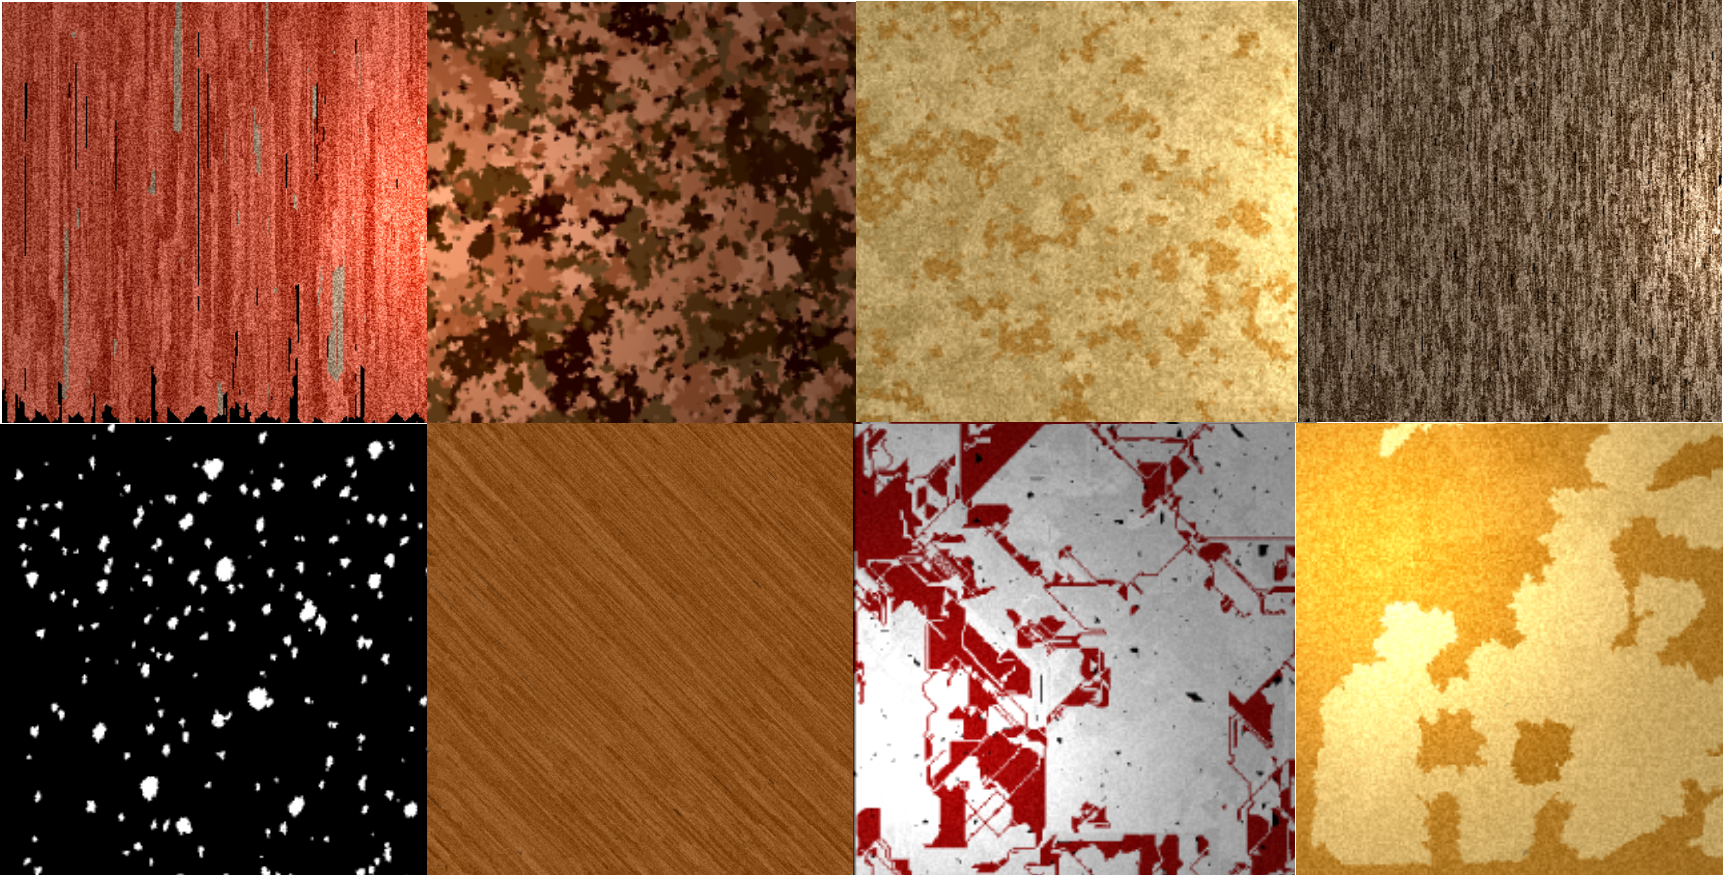
\includegraphics[scale=0.18]{resultados}
\caption{Textures obtained with Particle Systems generation.}
\label{resultados}
\end{figure}

The parameter setting for the texture in Fig.~\ref{sintesis} is:

\begin{itemize}
\item Parameter {\em amount of initial particles}, $100$.
\item Parameter {\em new particles per iteration}, $1$.
\item Parameters {\em color 1 and 2 (RGB)}. with example colors, one with a higher green component and other with a higher blue component.
\item Parameters {\em directions}: randomm: $50\%$, diagonal $50\%$.
\item Parameter {\em color variation}, $0.1$, in a scale of $[0,1]$ (see $varcolor$ in previous section).
\item Parameter {\em color variation per particle}, $0.1$, in a scalr of $[0,1]$, that determines the texel color variation inside the particle.
\end{itemize}

\begin{figure}[t!]
\centering
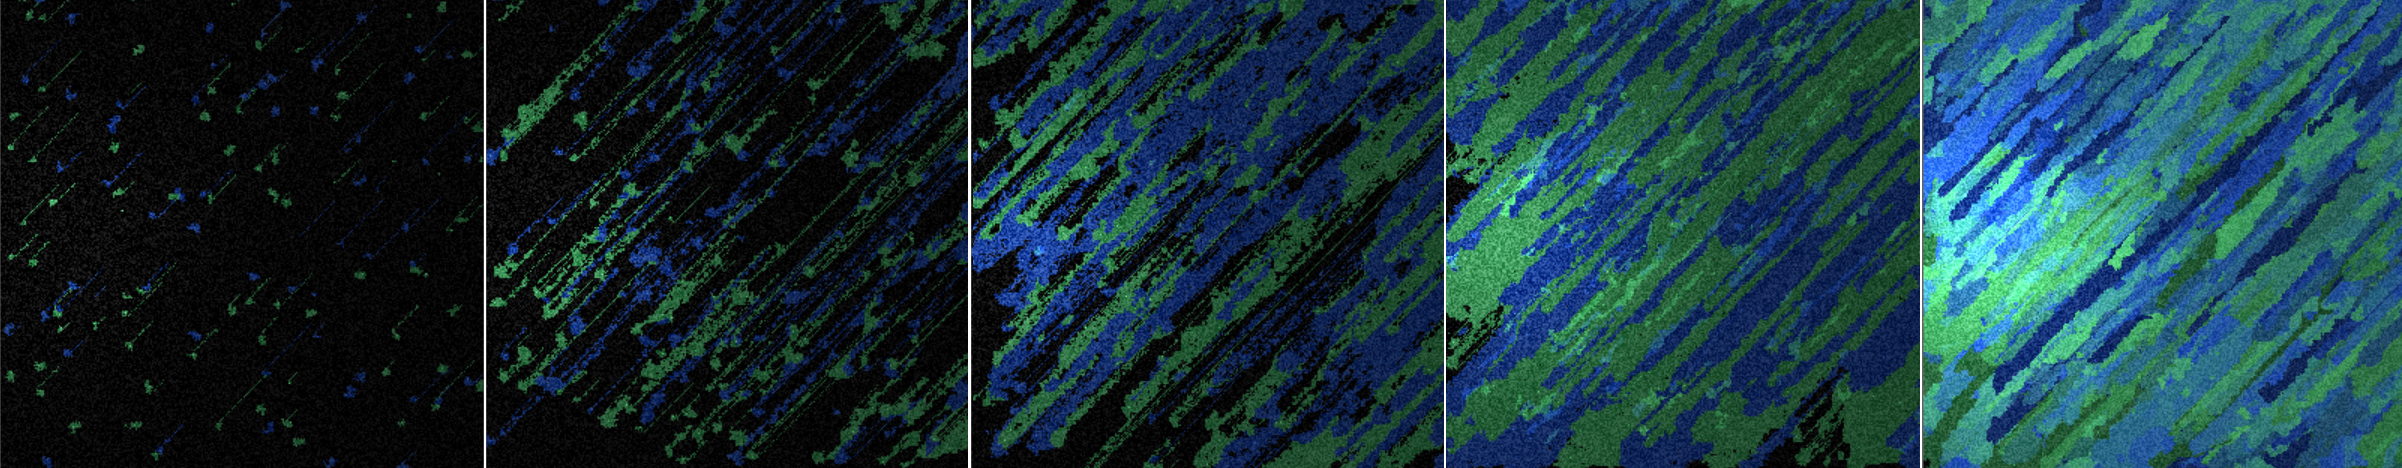
\includegraphics[scale=0.12]{sintesis}
\caption{Texture synthesis example.}
\label{sintesis}
\end{figure}

\begin{figure}[t!]
\centering
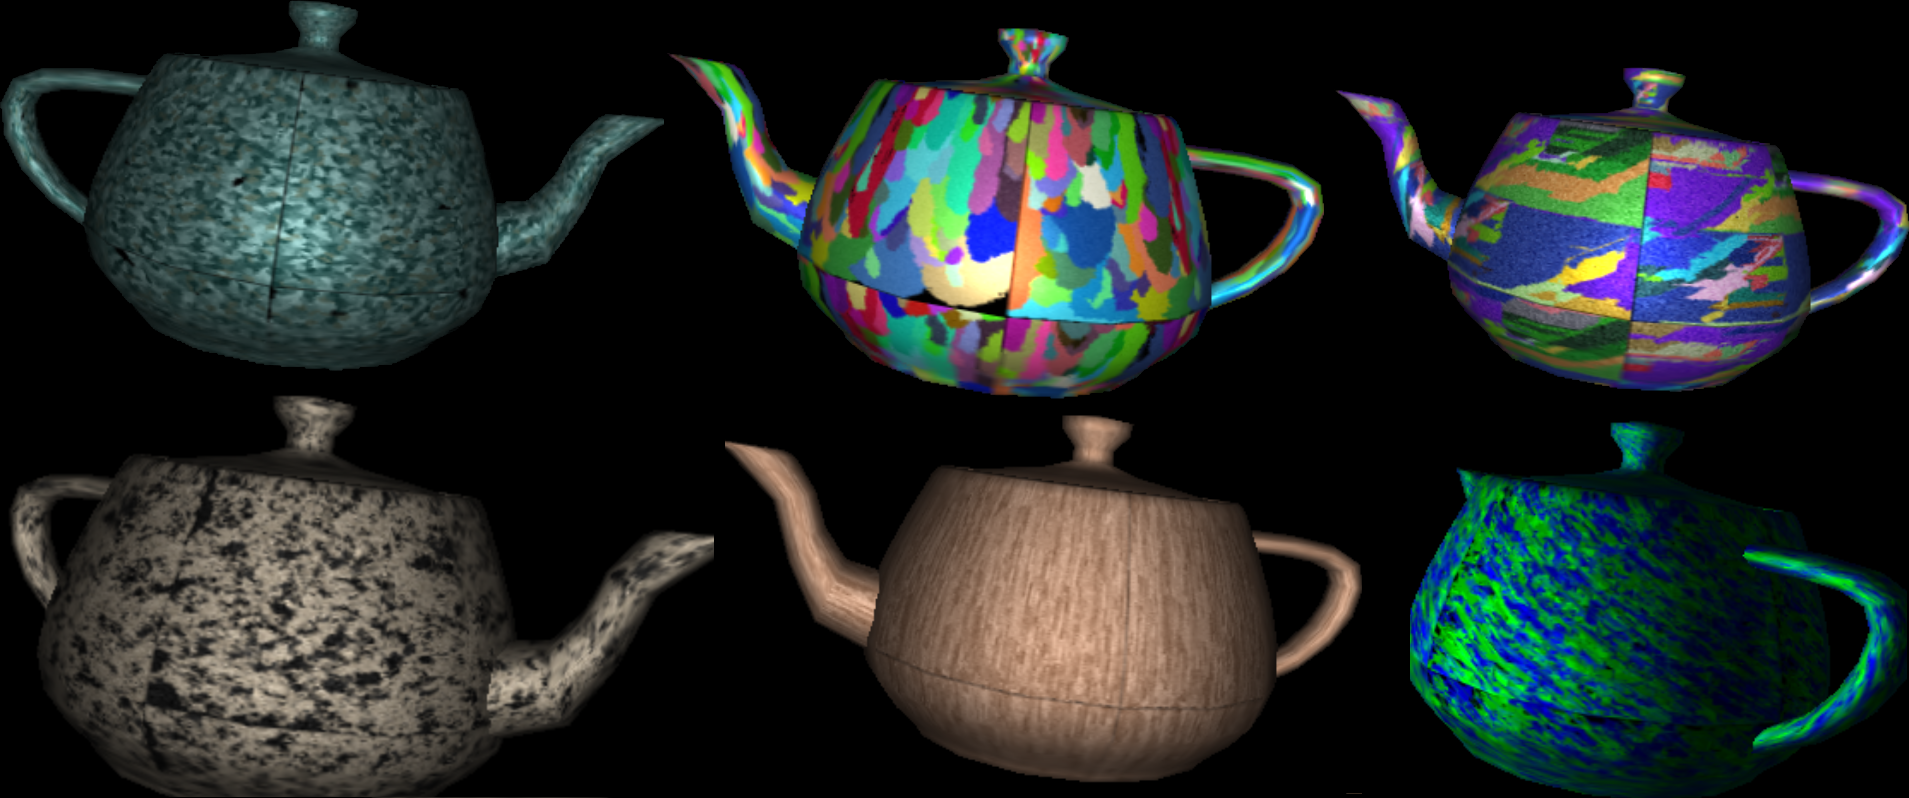
\includegraphics[scale=0.14]{teteras}
\caption{Generated textures mapped on a teapot.}
\label{teteras}
\end{figure}


\begin{figure}[t!]
\centering
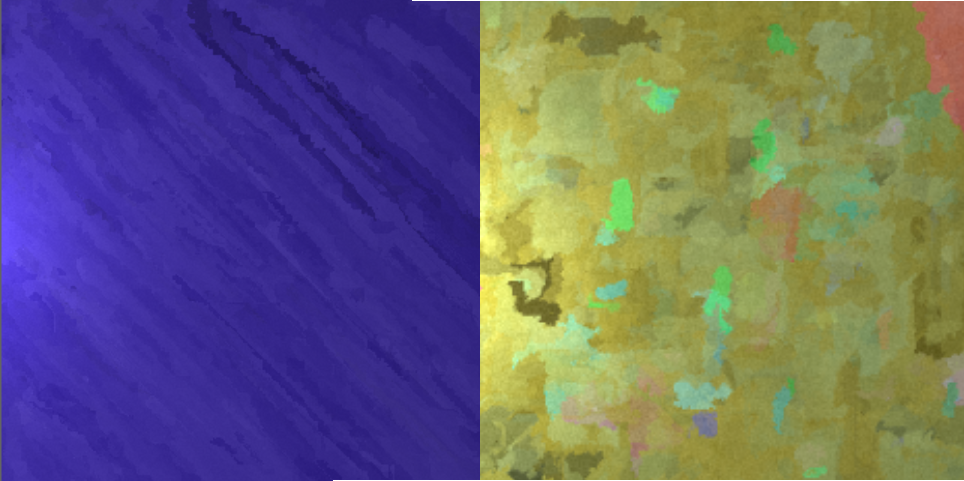
\includegraphics[scale=0.2]{muerte}
\caption{Texture using the death effect of particles.}
\label{muerte}
\end{figure}

The obtained results show high flexibility, useful to produce different materials.
We will develop the idea of using particle systems to produce materials in next section, more specifically, to produce the geometry of porous materials.
Results will be generalized to three dimensions.

\section{Procedural Modeling of Bread Crumb Geometry}
Here we introduce a procedural model to simulate the geometry of bread, based on the previous section.

Although the introduced model is not based on first principles, it is a step that will be refined to produce a more physical model in next section.

\subsection{Introduction}
The overwhelming variety of materials and their complex light interactions has been a central research topic in Computer Graphics for decades. 
Physics-based modeling may achieve outstanding light transport phenomena, whose computational approximations are a mainstream topic in the current research on rendering.
In complex materials, geometric modeling undergoes a similar research strategy, starting from a Physics-based understanding of the material that further leads to an adequate computational approximation.
Realistic material rendering should take into consideration geometrical modeling and light interaction simultaneously.

The choice of a geometrical model depends on the material and the intended scale representation.
This choice highly influences the rendering algorithm. Main approaches to material rendering include surface or volume treatment. 
The rendering equation \cite{Kajiya1986} models geometrical optics behavior in surfaces. 
The volume rendering equation \cite{Kajiya1984} represents scattering phenomena in volume densities.

Typically, authors use the surface representation for homogeneous materials (metals, plastics, and similar materials) \cite{Neumann1999}.
This method models microscopic surface details using statistical assumptions.
If mesoscopic details are modeled (as required for instance in wood or bricks) \cite{Lefebvre2000}, a usual technique is to precompute these details in textures that can be mapped onto surfaces.
Locally flat surfaces are fast to render but they impose limitations to the rendering quality that are sometimes impossible to surmount, specially the features that arise due to the mesoscopic structure and light transport phenomena in the materials.

Bread crumbs are extremely complex materials to model and render, due to the intricate geometries and light transport phenomena arising within them.
In this particular case, the naive surface approach flatly fails, since mesoscopic details, clearly visible on their surfaces, are essential to recognize the material.
More sophisticated surface modeling techniques, like the use of bidirectional texture functions \cite{Tong2002}, does not handle light propagation phenomena adequately.
To overcome this limitation, a complex material model is proposed \cite{Tong2005}.
This method produces more realistic results, but the capturing and rendering procedure are extremely complex, and the modeling is somewhat inflexible (for example, the surface representation does not allow arbitrary cuts).

On the other hand, there is a wide literature about modeling materials that are better fitted to a volume representation (for example smoke and clouds) \cite{Chentanez2011,Zhou2008}.
Volumes are computationally expensive but, being mesh-free, they do not have the rendering drawbacks mentioned above for surfaces.
There is a trade-off, then, between geometrical representations for complex materials.
Where simplicity and real-time rendering are required, surface-based representation is mostly used, and when photorealism is the final requirement, a volume-based modeling is chosen.
However, the arise of GPUs is shifting this trade-off, since it may allow volume representations at interactive time rates, as we show in this work.

In this section we propose a volume representation for bread crumbs.
Instead of computing voxel values using algebraic functions \cite{Perlin1989}, the crumb geometry is modeled using particle systems \cite{Reeves1983} in a $3D$ cube that evolves with dynamical systems \cite{Strogatz2001}, emulating the yeast behavior in dough.
This produces bubble distributions with controllable geometric and statistical properties that allow a photorealistic rendering of a variety of bread crumbs.

We apply direct volume rendering (DVR) \cite{Levoy1988,Kruger2003, Kratz2006} on a scalar field to render the final structure.
DVR applies a ray marching algorithm through a volume, accumulating different properties for each pixel.
We expand the ideas presented in \cite{Baravalle2014}, enhancing the rendering method with self-occlusion, specular highlights, automatic crust determination, and shadows, achieving more realistic images while reducing the overall computational cost at the same time.
The rendering workflow does not use intermediate structures, simplifying the modeling process.
In addition, the bread crumb shape can be modified interactively, with the possibility of performing arbitrary cuts and slices of the 3D structure in real time.
Also, the bread crust can be easily defined along with its own properties like color and translucency.

\subsection{Dynamical Systems as a Model of Bread Crumb}

This algorithm produces the underlying geometry for rendering.
Therefore, instead of delivering the color of a particular space position it will generate a scalar field composed of $0$s and $1$s ($0$: air, $1$: mass).
This representation is adequate for DVR.
The system consists of a set of particles $P$, 

\begin{equation}
  P = \{p_{1}, ... , p_{n}\}, n  \in \mathbb{N},
\end{equation}

\noindent a lattice $L_{N\times N \times N}, N \in \mathbb{N} $ (initially $L_{xyz}=1$) of mass and air, and a lattice $L^2_{N\times N \times N}$, (initially $L^2_{xyz}=-1$), of positions and particle ownership ($i$ if the lattice element belongs to the contour or interior of the particle $i$). 
Each element in $P$ has the following properties:

\begin{equation}
  p_{i} = \{O_{i}, C_{i}\}, 1 \le i \le n,
\end{equation}

\noindent where:

\begin{itemize}
\item $O_{i} = \{o_{1}, ... , o_{n_{i}}\}$: (Occupied) vector (set) of occupied positions by the particle in $L$.

\item $C_{i} = \{c_{1}, ... , c_{m_{i}}\}$: (Contour) vector (set) of positions representing the particle {\em contour} in $L$. 

\end{itemize}

The vector $O$ represents the positions affected by the particle, and the contour $C$ warrant avoidance with other particles. 
We describe in more detail the procedure in Algorithm $1$.
When $t = 0$, a set of particles take random lattice positions.
Each particle adds its position to $O$ and the surrounding positions to $C$.
In each iteration, each particle chooses a position on its contour. 
If the position lies in the contour of any other particle ($L^2_{position} <> i$ and $L^2_{position} > -1$), the process discards it and selects another contour position.
If that position is free ($L^2_{position} = i$ or $L^2_{position} = -1$), the particle adds the position to its $O$ and updates its contour $C$ and the lattices.
If the contour vector is empty, the particle {\em dies}, since it cannot grow anymore in the simulation.
Termination of the algorithm is possible at any $t$. The user can stop the simulation at a particular event, for instance, when the $L^2$ lattice is full ($L^2_{xyz} <> -1$ in any lattice position), since no progress can be made.

The method produces different structures varying the contour size ({\em separation} in Algorithm $1$, see Fig.~\ref{fg:fig1}). 

\begin{figure}
 \centerline{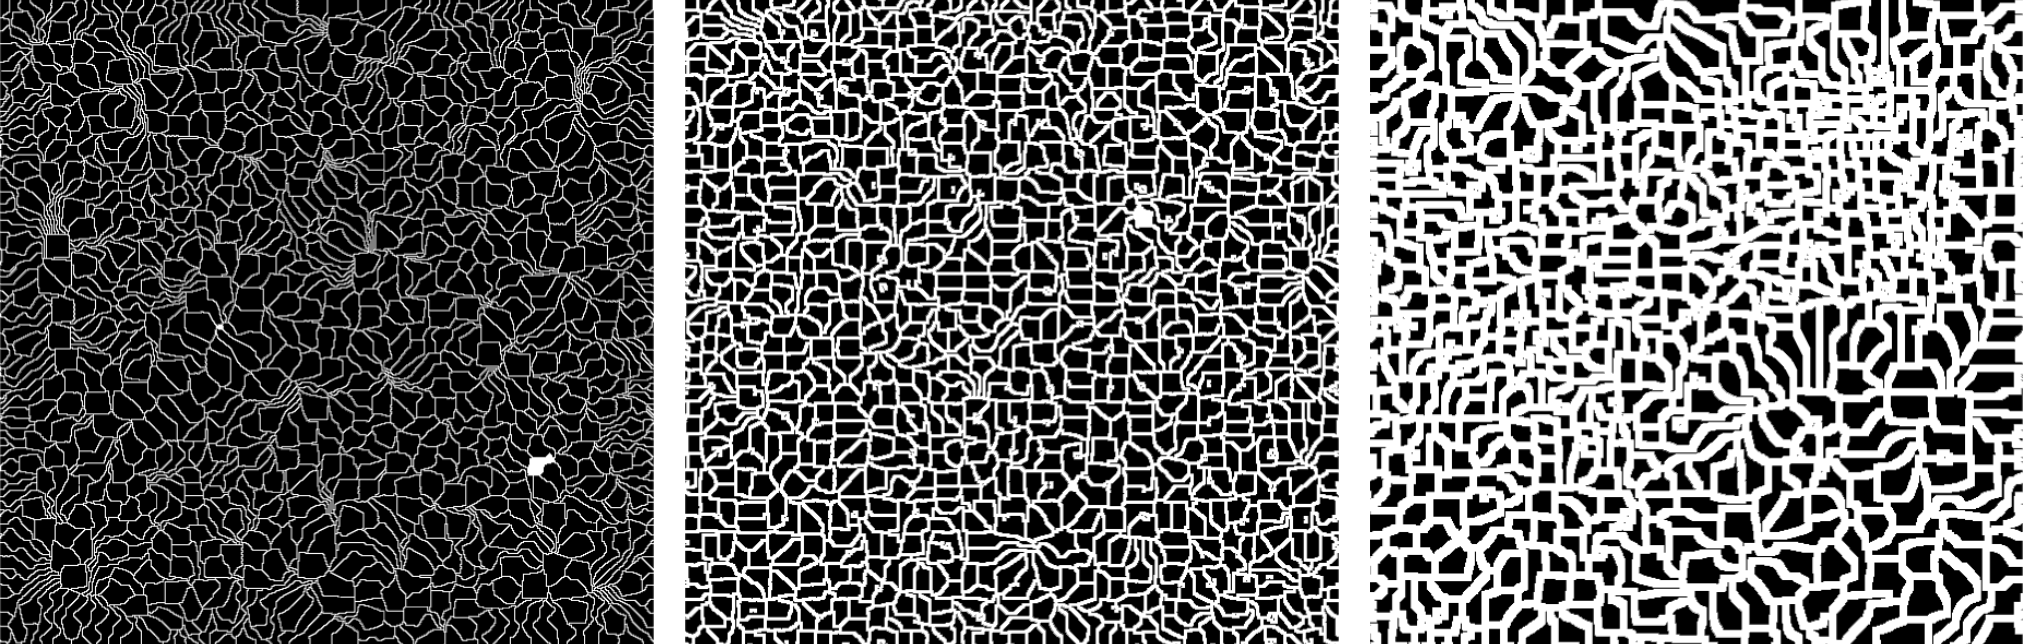
\includegraphics[width=13cm]{sistdin1}}
  \caption{Modeling algorithm, different values for the separation parameter. Left: separation = 1, middle: separation = 2, right: separation = 4.}
  \label{fg:fig1}
\end{figure}

Fig.~\ref{fg:fig1} shows 2D output examples (for better understanding) of random growing particles.
The contour size determines the white region among particles (mass) (the {\em width} of the white area). 
The resulting images seem to form Voronoi-like patterns.
The output of the algorithm is the lattice $L$.

\begin{algorithm}[ht!]
\caption{Modeling Algorithm}
\begin{algorithmic}

\State{$t  = 0, P  = []$}
\Comment{time (iteration), particles}
\State{$L  = matrix(MxMxM).init\_values(1)$}
\Comment {Geometry - initiated to 1 (mass)}
\State{$L^2 = matrix(MxMxM).init\_values(-1)$}
\Comment{Particle Domain}

\For{$i \in [1,particles\_count]$}
    \Comment{random position in L for each particle}
    \State{$x \gets random(), y \gets random()$}
    \State{$O[i] \gets [[x,y]]$,$C[i] \gets []$ }
    \For{$v \in neighborhood(x,y)$}
        \State{$C[i].add(v)$}
    \EndFor
    \State{$P.add([O[i],C[i]])$}
\EndFor

\For {$t \in [0,max\_time]$}
    \For {$i \in [1,particles\_count]$}
        \If {$empty?~C[i]$}     
            \State{die()}
        \EndIf
        \For{$h \in C[i]$}
            \State{$C[i].delete(h)$}
            \Comment{the position was explored}
            \If{$!(L^2[h] > 0 ~\&\&~ L^2[h] != i ~\&\&~ free\_boundary(separation))$}
                \State{$L[h] \gets 0$, $O[i].add(h)$} \Comment{mass $->$ air **}      \State{$C[i].add(neighborhood(h))$, $L^2.set(neighborhood(h),i)$} 
\Comment{Mark positions in $L^2$ as $i$}
                \State{$L^2.set(h,i)$}
            \EndIf
        \EndFor
    \EndFor
\EndFor
\end{algorithmic}
\end{algorithm}


\subsubsection*{Particle evolution using dynamical systems}

Human perception is very sensitive to patterns, in particular in bread crumb structure.
For instance, the eye immediately recognizes that the bubble shapes tend to follow the crust shape.
This effect is due to the fact that temperature in baking affects the bubbles' shape \cite{Scanlon2001}, stretching them following the crust.
Also, the entire structure has a fluid-like appearance.
Indeed, this is the case in early stages of the baking process.
At some point, the viscosity of the dough decreases and the bubbles stop growing and
coalescing.

Dynamical systems (DS) are a mathematical framework for understanding the dynamic behavior of
differential equations in dynamical processes \cite{Strogatz2001}.
Many dynamical phenomena can be described by defining differential equations that represent their behavior in time, simulating the evolution of the system and deriving approximate albeit useful solutions.
DS have been used in several domains for generating structures that resemble natural shapes.
A numeric integration of the equations starting from several initial conditions (or ``seeds'') gives rise to a set of streamlines.
For instance, the following equations produce Fig.~\ref{fg:fig3}(a):

\begin{equation} \label{eq:image_dynamics}  
  \begin{aligned}
    \dot{x} &= x^{2}-y^{2}+1,\\
    \dot{y} &= 2xy+1.
  \end{aligned}
\end{equation}

Figs.~\ref{fg:fig3}(b) and (c) are examples of other equations sets, where the resulting streamlines show different geometrical patterns.


\begin{figure}
  \centerline{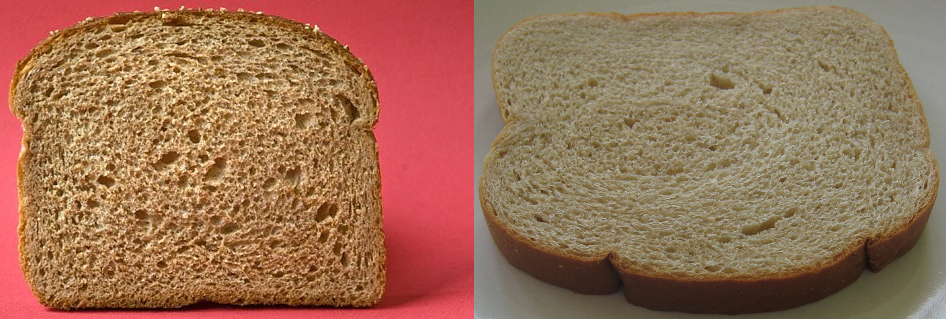
\includegraphics[width=13cm]{panreal}}
  \caption{Examples of dynamical systems in the plane used to simulate bread crumbs.}
  \label{fg:fig3}
\end{figure}

A DS can be used to ``drag'' information along the streamlines. 
In particular, in this modeling phase, we will use a DS to modify the underlying geometry of the particle system shown above.
The particles' final positions will be dragged along the streamlines of a DS that will alter the geometry, making it resemble the bubbles' deformation described above.
Algorithm $2$ shows the modification that we introduced to the original modeling algorithm.

\begin{algorithm}
\caption{Dynamical Systems Modification for the modeling algorithm}
\begin{algorithmic}
\State $L[h]\gets 0$ \Comment{mass $->$ air **}
\State $O[i].add(h)$
\State $solution \gets Runge\_Kutta(h)$
\Comment {Computes next position}
\State $neigh = neighborhood(h)$
\State $best = abs(neigh[0] - solution)$
\State $chosen = h$
\State $neigh.delete(h)$
\For {$w \in neigh$}
\State{// Best neighborhood solution that approximates the system}
    \If {$abs(neigh[w]-solution) < best$}
        \State $best = abs(neigh[w]-solution)$
        \State $chosen = w$
    \EndIf
    \If {$random() > 1-randomness$} 
    \Comment {$0 <= random() <= 1$}
        \State $C[i].add(w)$
    \EndIf
\EndFor
\State{// The best approximation is added}
\State $C[i].add(chosen)$
\end{algorithmic}
\end{algorithm}

Fig.~\ref{fg:fig4} shows particles following the DS streamlines, where the DS is the same as in Fig.~\ref{fg:fig3}(c).

\begin{figure}
  \centerline{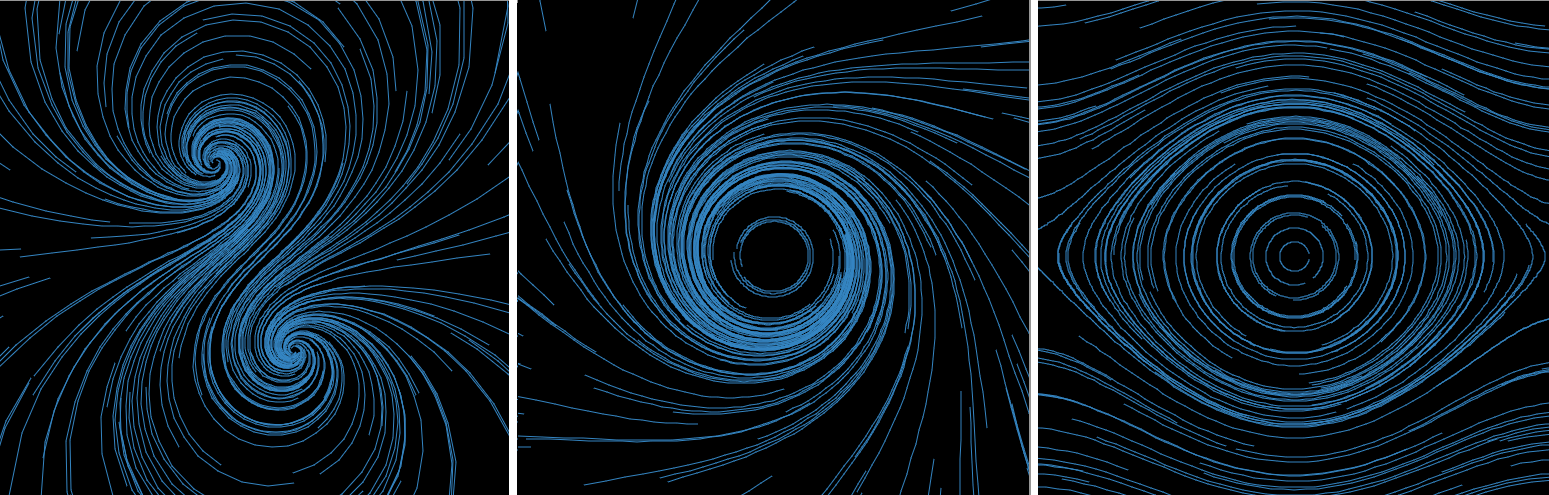
\includegraphics[width=13cm]{sistdin2}}
  \caption{Particle systems following dynamical systems . Effect of the randomness parameter. From left to right, randomness: 0.3, 0.2, 0.1 respectively. }
  \label{fg:fig4}
\end{figure}

From left to right, we decrement the trajectories {\em randomness}.
The randomness set to $0.1$ produces the right image, meaning that it forces bubbles to follow the DS trajectories with a probability of $0.9$.
We define this probability as $1-randomness$, with $0 \leq randomness \leq 1$.
The resulting patterns are now more similar to those arising in real bread and other baked foods.
We can define different useful structures employing different set of equations and different parameters for the particle systems (lifetime, randomness).

\subsubsection{Results and Limitations}
Figs.~\ref{fg:crumb} y \ref{fg:results2} show rendered images using our method.

\begin{figure}
  \centerline{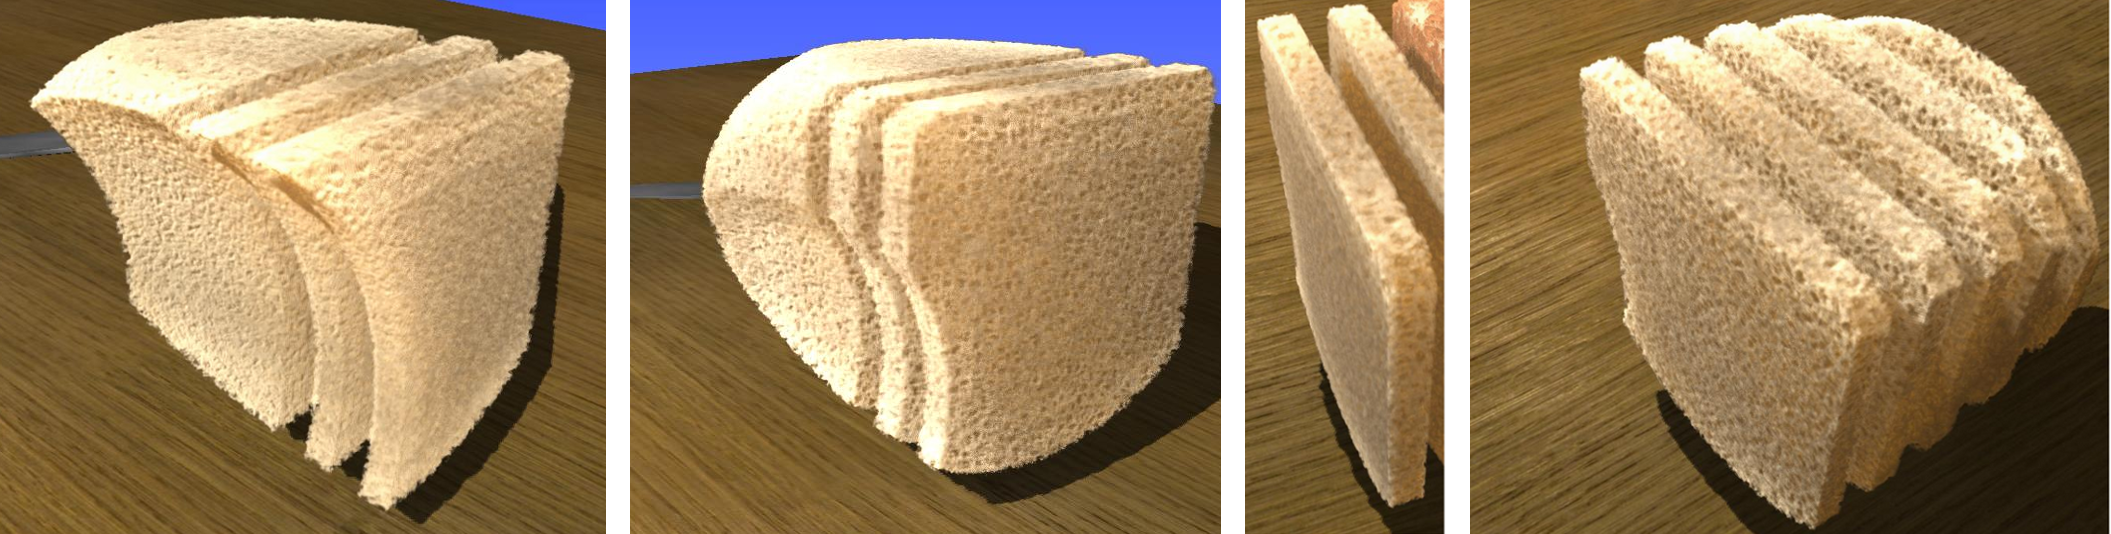
\includegraphics[width=13cm]{figures/crumb}}
  \caption{Rendered bread crumbs.}
  \label{fg:crumb}
\end{figure}

\begin{figure}
  \centerline{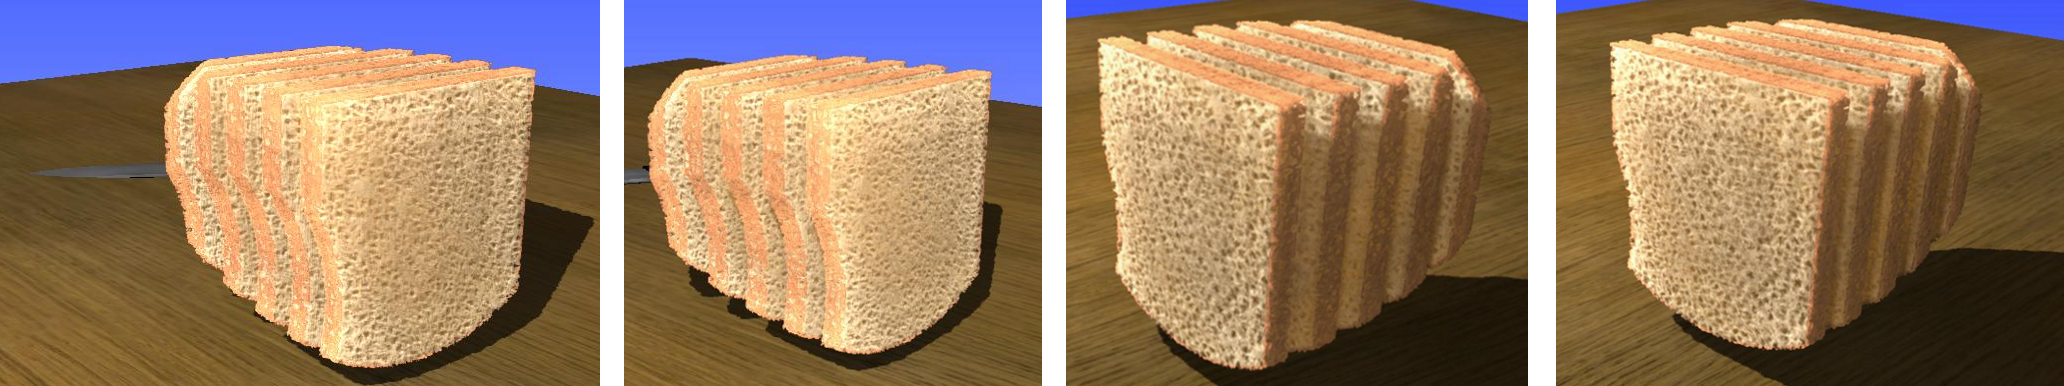
\includegraphics[width=13cm]{figures/results2}}
  \caption{Rendered bread crumbs with added crust to enhance perception.}
  \label{fg:results2}
\end{figure}


Even though it is possible to obtain different geometries in a simply and semi-automatic way, it is still difficult to generate arbitrary bread types.
The procedure relies in a dynamical system to produce the global bread shape.
The patterns generated by the system are difficult to tune.
Based on this, in the next section we present a more complete algorithm to fill these gaps.
It is also a volumetric method, but based on physical models imported from food engineering.


\section{Bread Modeling Using its Manufacturing Process}
In order to be able to realistically model the geometry of the bread crumb, it is necessary to tackle its physical development.


\begin{figure*}
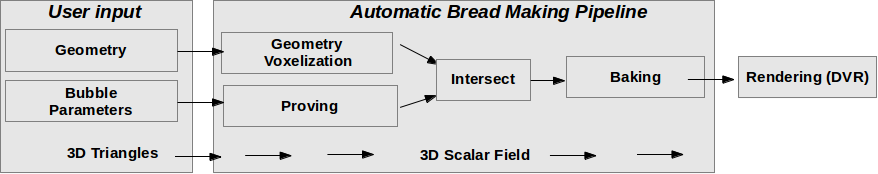
\includegraphics[width=13cm]{figures/pipeline}
\caption{Pipeline for synthetic bread making.}
\label{FigPipeline}
\end{figure*}

We propose another volumetric model for bread crumb and crust geometry generation.
In this section we will differentiate, and unify, the main steps of bread making (proving and baking).
These processes have been vaguely studied in the computer graphics literature.
First of all, we will review the state of the art in bread making.
Then we will present the modeling processes, that together with the illumination model of the next chapter, give rise to photorealistic images of several bread types.

\subsection{Previous Work}
Procedural modeling of geometry substantially reduces the need for artistic intervention in domains or situations where repetitive supervised action would turn out impractical, for instance in shaping cities \cite{Parish2001}, planets \cite{Ebert2002}, buildings \cite{Muller2006}, and plants \cite{Prusinkiewicz1990}. 
Some methods employ grammars to define mathematical descriptions that represent spatial relationships between primitives, for instance cubes, cylinders, or lines. 
The final structures usually arise using recursion over tokens in the grammar.

Although there was some initial research in computer graphics on bread crumb modeling and rendering \cite{Tong2005,Xenakis2007}, the overall process of bread making involves several stages that were not always well accounted for in the field.
Earlier works applied physical baking models to certain bread types for rendering animations ({\em e.g.} \cite{Rodriguez-Arenas2011}), but the bread crumb bubbles' geometric modeling issue was not considered.

Procedural bread modeling, on the other hand, is a multidisciplinary research subject.
Literature in food engineering has various decades of ongoing research aimed at understanding the bread production process. 
Studies in this area show that the proving stage of bread making strongly determines the features present in bread crumbs, in particular the bubbles \cite{Babin2006}.
The interaction between the yeast and some nutrients present in the dough produces {\em $CO_{2}$}. 
Bubbles' radii and their spatial distributions show fractal-like structures, exhibiting a distinguishable statistical self similarity at different measurement scales. 
Studies computed different fractal dimensions for these structures in certain bread types \cite{Gonzales2008}, suggesting uniform fractal bubble distributions. 
The bread baking modeling has also been subject of significant research \cite{Mondal2008}.

Procedural fractal representations for other materials arose a wide variety of research interests, including disparate topics such as mountains \cite{Prusinkiewicz1993}, moon craters, and bubble size distributions in cheeses \cite{Mandelbrot1982}. 
In addition, complex mathematical models represent the behavior and growing of several natural phenomena. 
In computer graphics, these models are one of the foundations used to model water and fluids \cite{Stam1999,Fedkiw2001}. 
Authors borrow complex differential models from other science fields, and compute them using numerical techniques. 
In recent years, GPGPU technology \cite{Owens2007} enabled the possibility of real-time or interactive frame rate computation and rendering of these numerical models.

Notwithstanding these breakthroughs, our final goal still presents several challenges. 
In addition to an accurate mesoscopic model (3D texture), bread crumb rendering requires an adequate representation of the light transport phenomena, including self-occlusion, self-shadowing, transmittance, and reflection, among others.
Only a few publications propose to manage both the geometric and illumination models, and mostly stressing only artistic considerations \cite{Xenakis2007}.  Also, these authors did not disclose enough details of the modeling and rendering algorithms (probably due to intellectual property issues) and thus the results are hardly reproducible.

On the other hand, the artistic community usually produces realistic bread rendering results using photographs and defining geometries from them, using translucent materials and subsurface scattering effects\footnote{http://www.blenderguru.com/tutorials/how-to-create-realistic-bread} and other ad-hoc considerations\footnote{http://design.tutsplus.com/tutorials/create-a-realistic-loaf-of-bread-in-photoshop--psd-10555}. 
While these solutions obtains very good outcomes, the processes are tedious and time demanding. 
Moreover, defining different bread models requires repeating the whole processes afresh, making the processes far from practical. 
The use of this way of modeling has several other drawbacks. 
For instance, it is not possible to get arbitrary slices of the resulting object.


\subsection{A Pipeline for Bread Modeling}
In relation to the previous work mentioned above, we propose to unify and differentiate the key steps of bread making (proving and baking) to produce a physically inspired pipeline for procedural generation of bread crumb and crust geometries.
These processes have to be well understood before an accurate modeling can be developed.

In this Section we describe all the stages that lead to the final rendering of a realistic bread material.
First, we review the state-of-the-art knowledge of the bread baking process, and we briefly introduce some ancillary mathematical models that will be required for understanding the main computational developments presented in this paper. 
Then, we present the modeling procedures that, together with the illumination model, give rise to the main results presented in this paper.

The whole process is comprised in a modeling pipeline (see Fig.~\ref{FigPipeline}), where all the stages emulating bread making are processes applied to scalar fields.
The user can feed the pipeline with a $3D$ model of their preference, or allow the system to provide standard shapes, usual in bakeries.
This geometry is voxelized in order to proceed.
During the bread proving simulation, the user can parameterize the texture of the dough (related to the amount and size of the bubbles), or, again, leave the default parameters that lead to a generic texture and appearance.
The dough will be intersected with the voxelized geometry in the previous step to obtain a final scalar field with the external shape provided by the user and with its interior filled with the bread material (see Section~\ref{breadprov}). 
Then a specific baking model is computed  \cite{Powathil2004} to slightly twist the scalar field (and the bubbles therein) according to the effects that baking produces in the bread making process. 
Finally we apply direct volume rendering (DVR) \cite{Kruger2003} to the final scalar field, obtaining realistic images of the resulting bread.

%====================================================================

\subsection{Geometry voxelization}

Users can generate arbitrary $3D$ bread shapes using our pipeline.
The first step voxelizes a user-provided model with the open source {\tt binvox} utility\footnote{http://www.cs.princeton.edu/~min/binvox/} \cite{Nooruddin2003}.
The voxelization generates a binary scalar field, where $1$ represents that the given voxel is inside the geometry, and $0$ means the voxel is outside.
In the proving simulation step (next subsection), we generate the texture of the material that lies inside this voxelized model.
This allows to generate arbitrary bread types such as {\em baguettes}, {\em croissants}, {\em sliced} breads, or fancy shapes.

An important sub-product of the geometry matrix is a secondary scalar field that can be obtained by means of the distance transform.
This transform generates a $n$-dimensional matrix of the same dimensions as the matrix being transformed \cite{osh03}. 
The transformation computes, for each matrix entry, the distance to the closest zero entry in the original matrix.
Given a binary $n$-dimensional matrix $M$, the algorithm generates a real valued matrix $DF_{M}$ with the same dimensions as $M$ in the following way,

$$  DF_{M}[i] = \min \bigg\{ \delta(i,j): M[j] = 0 \bigg\},$$


%\[
%distField(M)[i] =
%\begin{cases}
%min(d(i,j)), & \text{if } M[i] != 0, \forall j \, M[j] = 0;\\
%0, & \text{otherwise, }\\
%\end{cases}
%\begin{align*}
%M'[i] &= min(d(i,j)), M[i] != 0, M[j] = 0\\
%M'[i] &= 0, M[i] = 0,
%\end{align*}

\noindent
where $i$ and $j$ are cells in the respective matrices, and $\delta(i,j)$ is the Manhattan or the Euclid distance between two cells in the underlying $n$-dimensional space. 
Matrix entries far from the object boundaries get higher values than entries closer to the boundary, getting a map of the distances to the object surfaces. 
This distance field will be required later at two different stages of the pipeline.

\subsection{Proving simulation}
\label{breadprov}

As stated above, the actual texture of the bread dough is due to bubble patterns, which in turn are the result of complex processes, including chemical reactions and physical deformations in the dough.
The proving step accounts for the free bubble growth produced by living yeast in the dough.
Then, human intervention deforms dough shapes in several ways, and the baking process gives the final bubble shapes.
Phenomenological studies of bubble distribution employ X-ray tomography devices and image feature extraction \cite{Babin2006,Gonzales2008,VanDyck2014}.
To obtain a similar structure variability, we generate bubble distributions with a fractal-based model inspired in the cheese and moon crater distributions proposed in \cite{Mandelbrot1982}, and we further validate it using the sandbox multifractal spectrum, as will be thoroughly explained later.

The texture of the dough is procedurally created in a separate $3D$ scalar field defined within a $3D$ matrix, in a similar way as the geometry matrix in the previous subsection.
Each cell is initially set to $1$ (meaning that the material has no bubbles so far).
The process begins by subtracting randomly positioned spheres of radii $r_{min}$ to this scalar field (by setting the respective cells to $0$).
Then, larger spheres will be subtracted, also at random positions, up to a maximum radius $r_{max}$.
The relationship between the amount $N(r)$ of spheres to be subtracted to the material at each step, and their respective radii $r$, is given by the following fractal law,

\begin{equation*}
N(r) = \frac{k}{r^{d}},
\end{equation*}
where $d$ is the fractal exponent that models the likelihood of occurrence of spheres in relation with their radii, and $k$ controls the amount of actual spheres at each radius. 
Both parameters are sufficient to model a wide range of textures in general, and bread textures in particular.

Fig.~\ref{FigProving} shows a $2D$ slice of this model.
Even though the resulting spherical bubble shapes are not completely realistic (for instance, the spherical nature of the bubbles is apparent and artificial), the results show high resemblance in size and distribution with real bread binarizations (see \cite{Babin2006}).
During baking, the resulting scalar field will undergo geometric deformations, and therefore the final texture will resemble actual bread more accurately.
Also, the issue of finding adequate parameter values to obtain features similar to real bread crumbs will be further discussed in the validation section.

\begin{figure}
\center
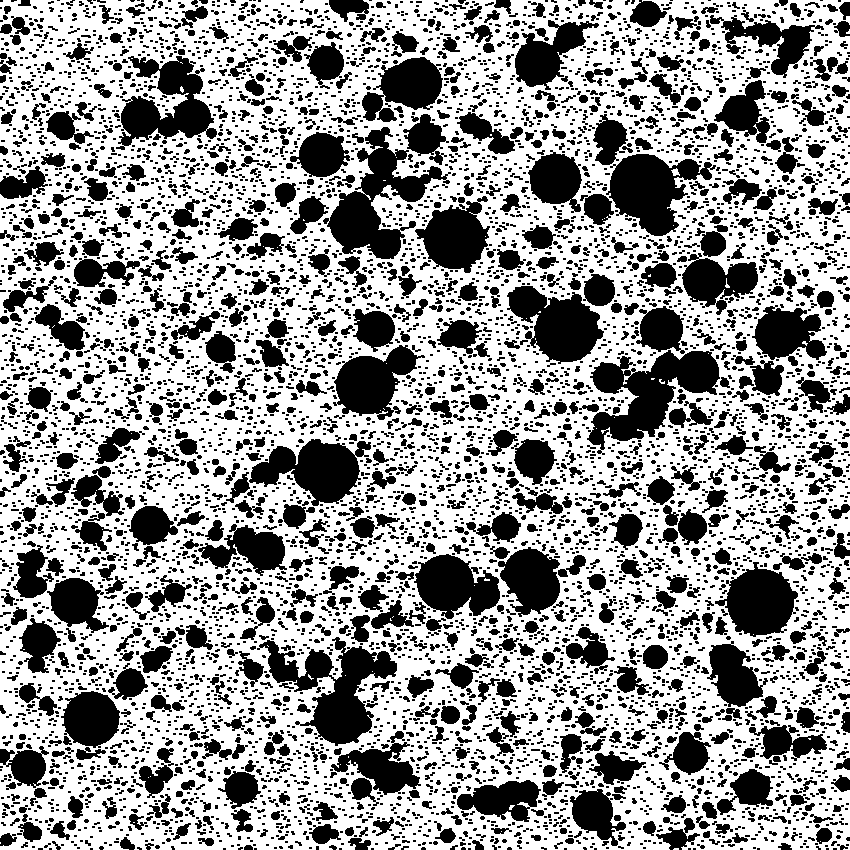
\includegraphics[width=8cm]{figures/bubbles}
\caption{Fractal bread proving simulation.}
\label{FigProving}
\end{figure}

After the voxelization and the proving simulation, we must constrain the dough to the interior of the geometry. 
For this, a na\"ive solution would be to intersect the two scalar fields by means of a simple product or masking:

\begin{equation*}
P_{2} = P_{1} * G,
\end{equation*}
%
where $P_{1}$ is the $3D$ field (matrix) containing the bubbles and $G$ is the scalar field representing the voxelized geometry. 
Fig.~\ref{fg:intersectProblem} shows some results of this na\"ive procedure.

Even though these results might appear satisfactory, actually bubbles are seldom present at the surface of real bread, due to some complex processes during proving (the exterior of the dough gets dehydrated, and therefore the yeast is unable to form CO$_2$ bubbles).
This process is not completely understood, and to account for it, the distance field computed at the previous stage is used to disallow bubbles to be generated close to the geometry's boundary. 
Bubble subtraction, then, is constrained to occur only when the outermost part of the bubble is within a given threshold distance to the external boundary of the shape.
%The resulting binary scalar field is computed as follows.

\begin{figure*}
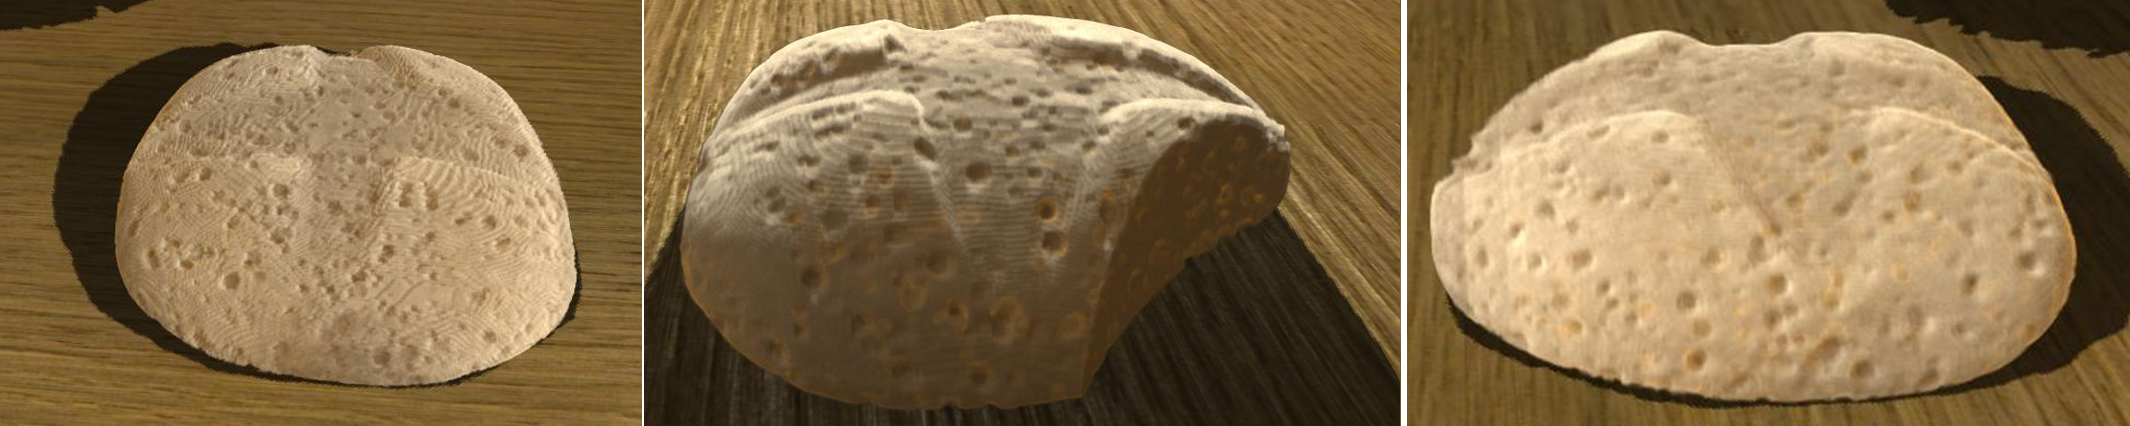
\includegraphics[width=13cm]{figures/intersectProblem}
\caption{Na\"ive geometry and bubbles intersection. Bubbles are unrealistically visible on the dough surface.}
\label{fg:intersectProblem}
\end{figure*}

%\begin{align*}
%DF    &= distField(G),\\
%inner &= DF > threshold,\\
%dough &= G - inner*(1-P_{2}),
%\end{align*}
%
%where $DF$ is the $3D$ distance field to the surface of the voxelized input geometry and $threshold$ is a value determining the outer region's width.
%The final dough is computed by subtracting the bubbles ($1-P_{2}$) from the original geometry, but limited to the computed {\em inner} region.

Figs.~\ref{fg:proving} and \ref{fg:provingBunny} show the result of limiting the bubble interactions to the inner region of the original geometry.
These images show that the approach also allows to produce realistic arbitrary unbaked doughs.
Note that our model is flexible enough to render the material at any stage of the pipeline, and also to arbitrarily slice or intersect the model.

\begin{figure*}
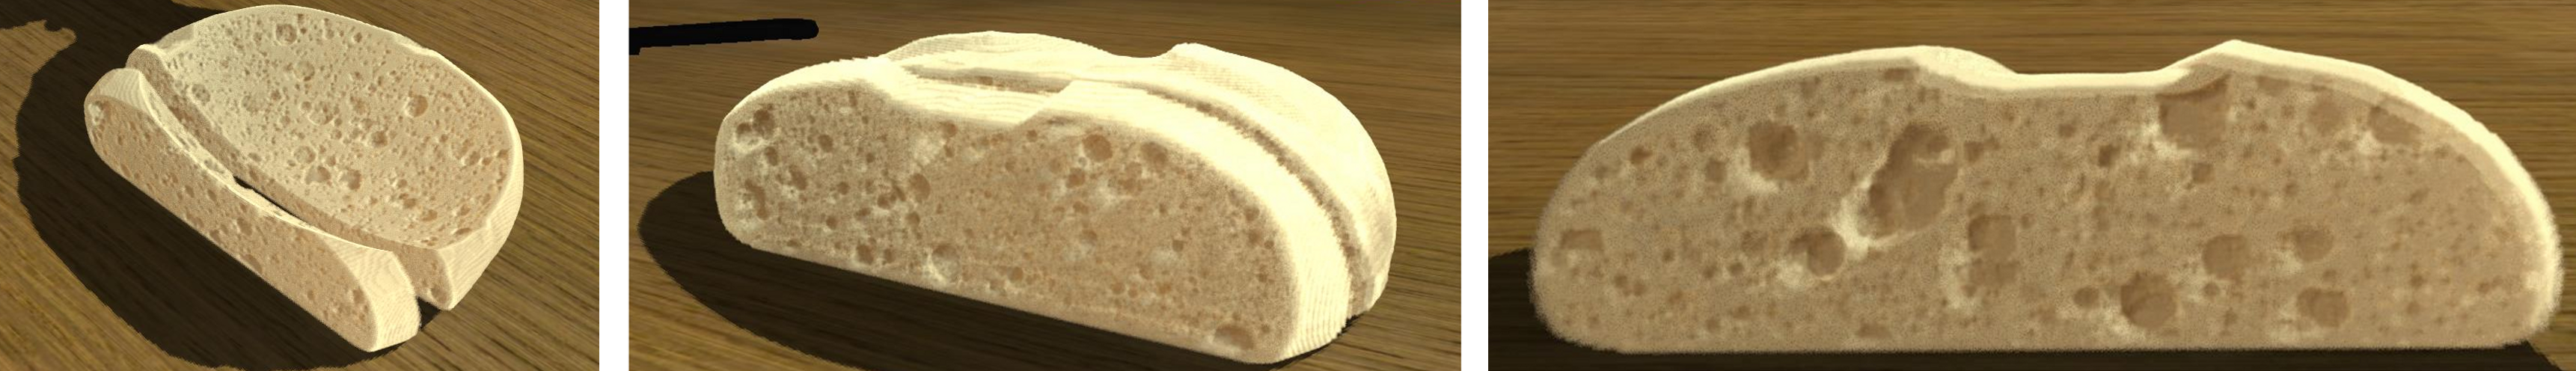
\includegraphics[width=13cm]{figures/prebakebread}
\caption{Proved bread before baking.}
\label{fg:proving}
\end{figure*}

\begin{figure*}
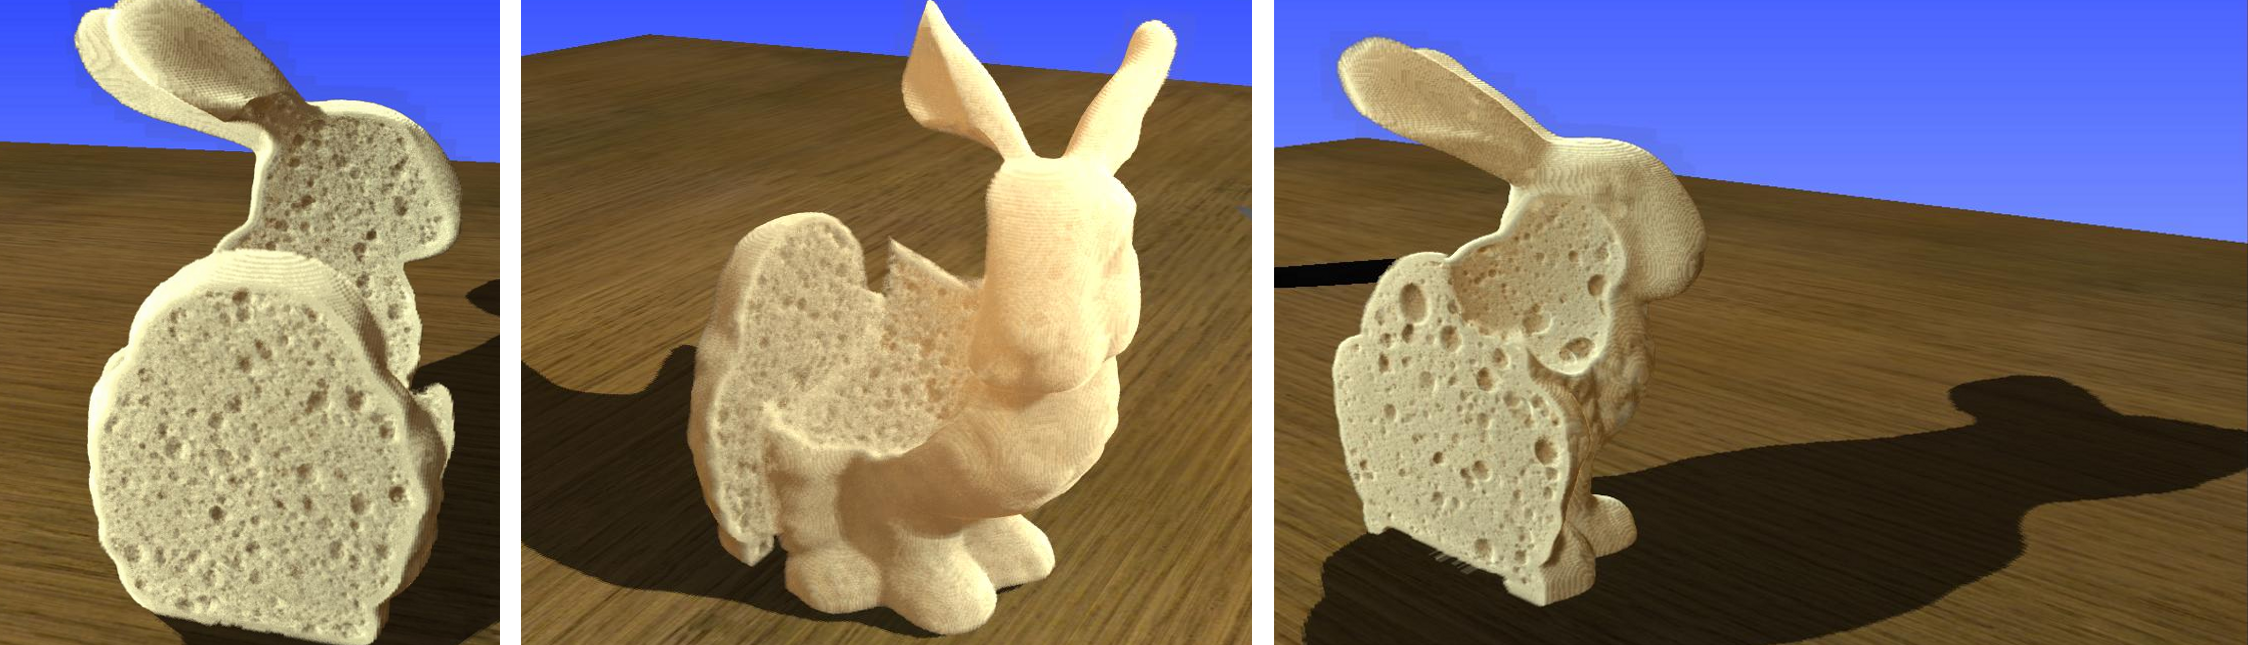
\includegraphics[width=13cm]{figures/prebakebunny}
\caption{Proved bunny-shaped bread before baking.}
\label{fg:provingBunny}
\end{figure*}

%====================================================================
\subsection{Baking}
%To adequately simulate the bread baking process, mathematical models should be able to accurately model the heat and mass transfer in dough.
Adequate physical models of the bread baking process should be able to accurately model the heat and mass transfer in dough.
Full $3D$ bread baking models may lead to precise solutions to the temperature's distribution in dough during baking.
However, these models are usually very complex to implement and they have high computational costs.
In addition, only the most complex models take into account the crust formation, but usually using overly simplified assumptions.
This is due to the fact that a formal crust definition is currently missing~\cite{Vanin2009}.

The most relevant results suggest that a $1D$ model could suffice for most purposes. 
For instance, Purlis~\cite{Purlis2011} models bread baking as a 1D problem, representing it as an infinite cylinder.
Other frameworks assume only one radial coordinate, resulting also in 1D models~\cite{Powathil2004, Thorvaldsson1999}.  
These works show that employing a simple 1D representation produces almost identical results on the  bubble shape deformation, as compared to the ones using higher dimensions. 

The numerical simulation that we implemented is based on the finite-differences foundation proposed by Powathil~\cite{Powathil2004} and Thorvaldsson and Janestead~\cite{Thorvaldsson1999}. 
The framework presented consists of a set of three coupled equations describing heat transfer, water vapor diffusion and liquid water diffusion.
In our algorithm, we require only the computed temperatures ($T$) as the input for the next stages.
Equation~\ref{Eq:heat} models heat transfer in bread dough, accounting for energy balance and water evaporation due to temperature~\cite{Thorvaldsson1999}:
%
\begin{equation}
\label{Eq:heat}
\frac{\partial T}{\partial t} = \frac{1}{\rho C_{p}} \frac{\partial}{\partial x} \left ( k \frac{\partial T}{\partial x} \right ) + \frac{\lambda}{C_{p}} \frac{\partial W}{\partial t}+\frac{\lambda W}{ \rho C_{p} }\frac{\partial \rho}{\partial t},
\end{equation}
%
where $T$ is temperature, $x$ is the radial coordinate, $t$ is time, $C_{p}$ is the specific heat, $\rho$ is density, $k$ is thermal conductivity, $\lambda$ is the latent heat of evaporation of water, and $W(x,t)$ is the liquid water content. 
The initial conditions
%
\begin{align*}
T(x,0) &= T_{0}(x), 0\le x \le L/2,
\end{align*}
and the boundary conditions (continuity and smoothness) define the model:
\begin{align*}
\left ( \frac{\partial T}{\partial x} \right )_{x=L/2} &= 0 , t > 0 \\
-k \left ( \frac{\partial T}{\partial x} \right )_{x=0} &= h_{r}(T_{r}-T_{s}) + h_{c}(T_{air}-T_{s}) - \lambda \rho D_{w} \left (\frac{\partial W}{\partial x} \right )_{x=0}
\end{align*}
%
where $h_{r}$ and $h_{c}$ are subterms of the heat transfer coefficient ($h = h_{r}+h_{c}$), $T_{air}$, $T_{s}$, $T_{r}$ are the temperatures in the surrounding air, at the surface of the bread and at the radiation source, respectively, $L$ is the bread height ($x = L/2$ is the bread center and $x = 0$ is the bread boundary), $D_{w}$ is liquid water diffusivity, and $T_{0}$ is the initial temperature. 
Temperatures are expressed in Kelvin ($K$). 
The model presents similar equations for water vapor diffusion ($W$) and  liquid water diffusion ($V$). 
Further details of this model can be found in \cite{Thorvaldsson1999}.
We use this model to obtain a map of temperatures at the end of the baking process. 
These temperatures will in turn affect the bubbles' shapes and sizes.

The baking simulation sets an oven at a typical baking temperature (by default we take $210^{\circ}C$) and discretizes time in intervals of $\Delta t = 30s$, and from the simulation we obtain an array $Temp$ of $N_{grid}$ temperature values. 
For numerical stability, we set $N_{grid}=32$ and we interpolate the temperatures to obtain higher resolutions ($N_{int}$). 
%Each value represents a dough position after $M$ baking time steps. 

The vector we obtained from baking has decreasing temperatures from $R = 0$ to $R = L/2$, as the center and the boundary of the bread have the lowest and highest temperatures respectively (heat transfer flows from the boundary to the center). 
We can use the previously computed distance field in conjunction with the temperature vector to map distances to temperatures. 
This allows us to define temperatures in the scalar field in a way that is compatible with a $3D$ baking simulation. Based on these considerations, we map the temperatures vector $Temp$ into $3D$ coordinates using the following relationship:

\begin{equation*}
\displaystyle R(x,y,z) = Temp[ round( DF(x,y,z) ) ], 
\end{equation*}
%
where $R$ is the resulting scalar field, and $x$, $y$ and $z$ are $3D$ coordinates in $R$. When $DF(x,y,z) = 0$, the $3D$ position lies at the boundary of the geometry, and $Temp[0]$ is mapped to $R(x,y,z)$. 
When $DF(x,y,z) > 0$, a lower temperature is mapped to $R$, since the position lies in the geometry's interior. 
Fig.~\ref{fg:baking} shows slices of the result of this mapping ($R$), using temperatures from an arbitrary baking time step in the three Cartesian planes. 
The images are almost identical to what will be obtained with a $3D$ simulation~\cite{Purlis2010}.

\begin{figure*}
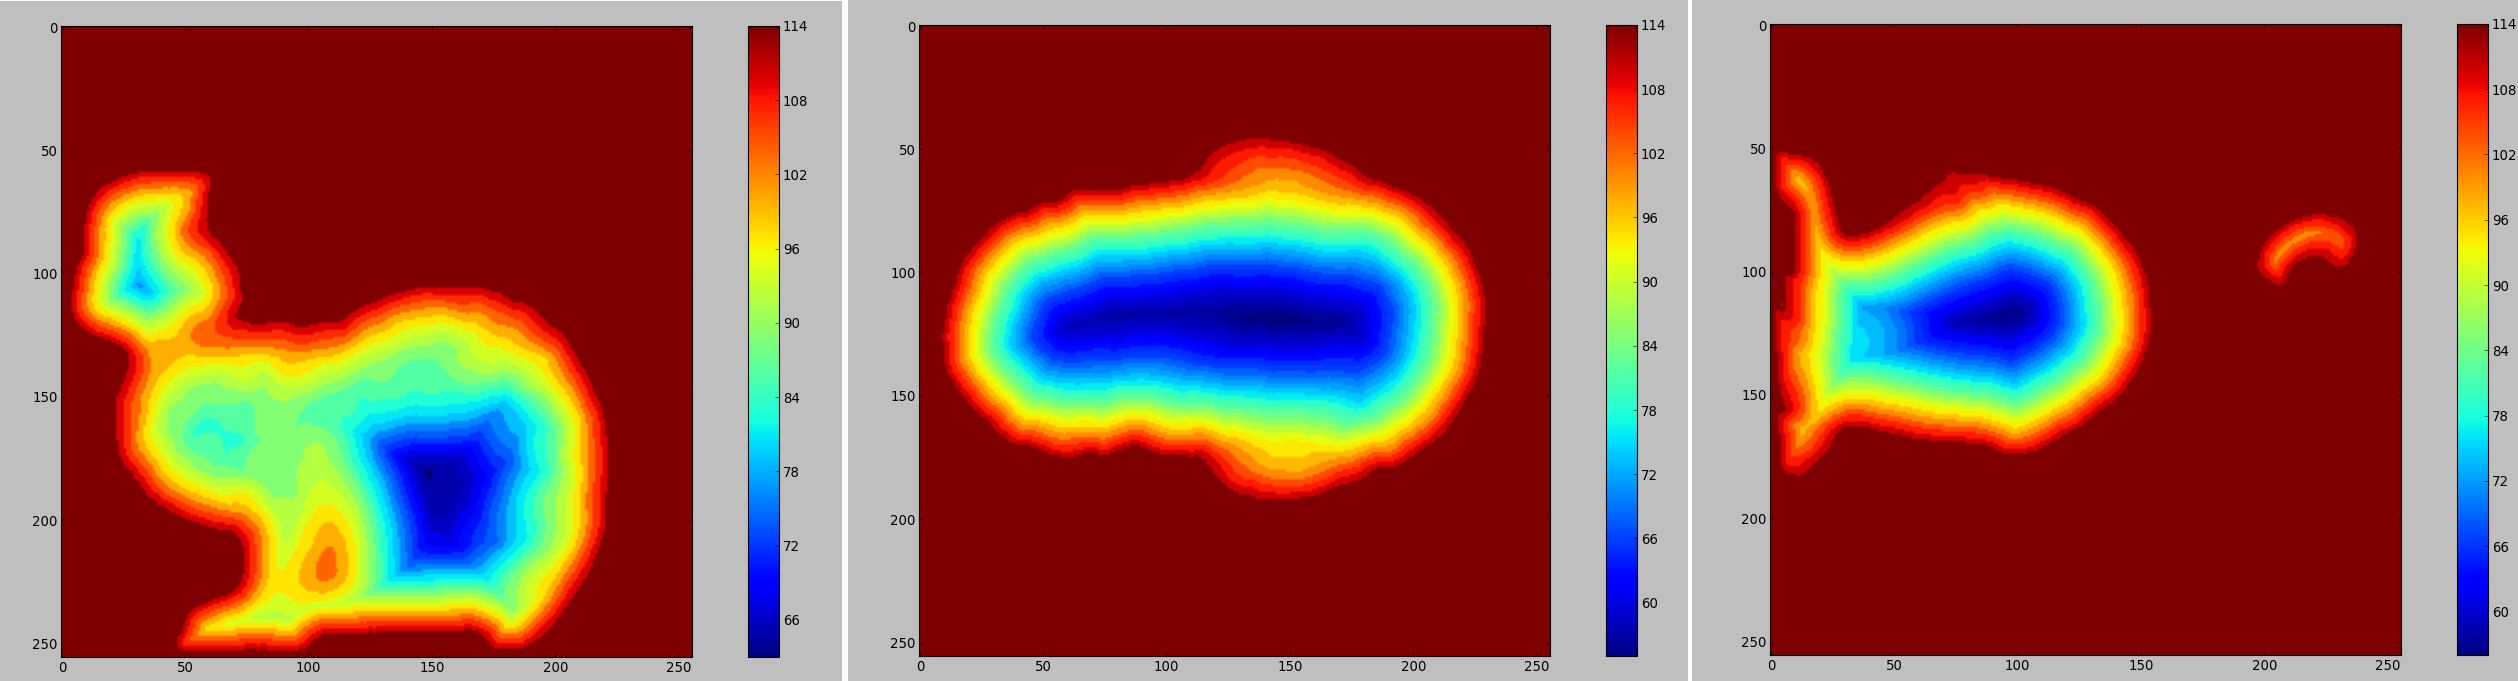
\includegraphics[width=13cm]{figures/tempsbunny}
\caption{One dimensional temperatures mapped onto a bunny-shaped $3D$ scalar field. The images show that temperature results similar to a complete $3D$ simulation.}
\label{fg:baking}
\end{figure*}

After a number of simulation steps (up to $t=20$ in our case), we compute the gradient vector field $g$ of $R$ \cite{Gonzalez2006}, and we smooth these fields using a Gaussian kernel.
We use the Gaussian smoothed versions to warp the original scalar field in the following way:
\begin{align*}
\displaystyle
u &= x+p*g'_{x}[x,y,z],\\
v &= y+p*g'_{y}[x,y,z],\\
w &= z+p*g'_{z}[x,y,z]
\end{align*}
where $(u,v,w)$ are the coordinates in the warped scalar field, ($x,y,z$) are the original field coordinates, $p$ is a real positive valued parameter that denotes field intensity (it controls the baking effect on bubbles) and the $g'$s are the smoothed Gaussian version of the original gradient $g$.
%Fig.~\ref{FigBakingVectorField} also shows the computed gradient, where using $[-g_{x},-g_{y}]$ produces a similar vector but in the clockwise direction that can be applied with similar effects on the bubbles. 
Fig.~\ref{fg:bakedbubbles} shows $2D$ scalar field slices with the baking process applied to different bread shapes.

\begin{figure*}
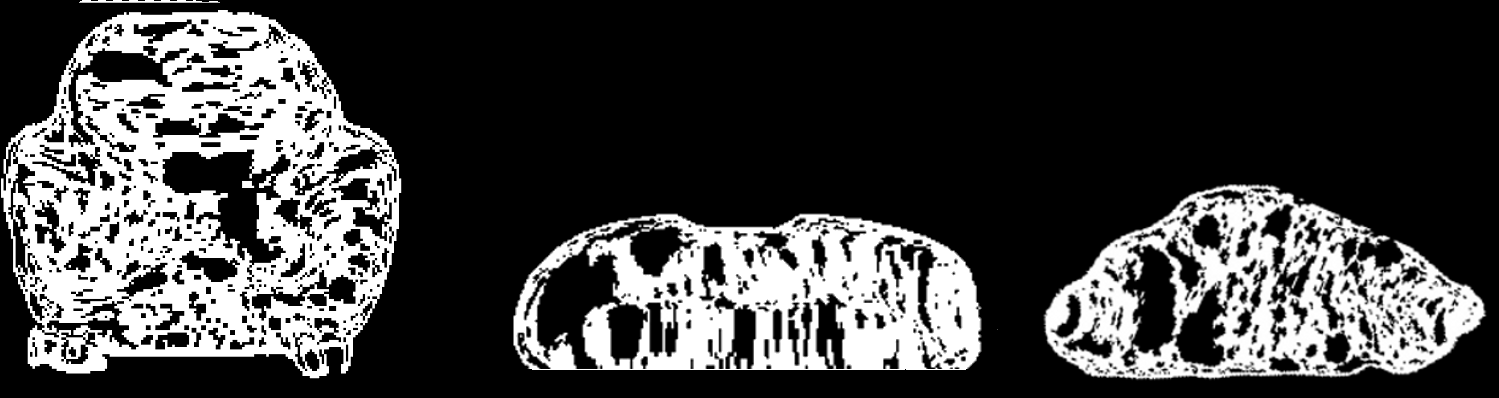
\includegraphics[width=13cm]{figures/bakedbubbles}
\caption{Two dimensional cuts showing bubbles after baking over different shapes.}
\label{fg:bakedbubbles}
\end{figure*}

The $p$ parameter can be used to synthesize different bread crumb appearances, from non-baked to highly deformed bubbles (see Fig.~\ref{fg:parameterp}).
When we increment $p$, we force the bubbles to follow more tightly the bread outer shape. 
The image also shows that the method deforms more intensely bubbles closer to the surface.

\begin{figure*}
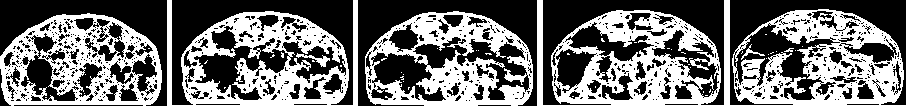
\includegraphics[width=13cm]{figures/parameterp}
\caption{Effect of the $p$ parameter: from left to right $p$ is $0$, $5$, $10$,$15$,and $25$, respectively.}
\label{fg:parameterp}
\end{figure*}


\subsection{Crust formation}

The baking model we introduced does not include precise details of the crust formation. 
In these equations, the crust is assumed to be produced in the surface and at certain temperature, but this assumption is far from what actually happens in the real baking process. 
The food engineering literature defines the crust as an interface that appears between the dough and the surrounding air.
Its main characteristics include the formation of a thicker material at the dough surface, and color differentiation, but the precise details surrounding the crust formation and appearance are still far from known.

Based on this initial approximation, we take advantage of the distance field that was previously computed to define a crust region.
We based this choice on the fact that the crust is mostly determined by an evaporation front that is result of the temperature \cite{Jefferson2007}. 
In other words, we obtain crust positions using the distance field, since we have defined a relationship between temperature and distance to the surface.
We use a distance parameter to obtain different thicknesses for the crust, getting different bread appearances.

%This is illustrated in Figure~, where arrow lengths indicate vector modulus. The image shows that the field's influence is higher near the crust, mostly deforming outer bubbles. This behavior is consistent with real bread crumbs: baking influences the outer bubbles' shape, elongating them parallel to the crust \cite{Scanlon2001}, in other words, following its isotherms.

\subsection{Rendering}
We applied Direct Volume Rendering (DVR) \cite{Kruger2003,Levoy1988, Max1995} to obtain the final images. %, as suggested in \cite{Baravalle2014}.  
DVR approximates the light transport equation by throwing rays from a virtual camera into a volume defined by a discrete $3D$ density function, accumulating density information and providing a $2D$ representation.
DVR samples the density function along the ray to approximate the effect of different light phenomena such as extinction, transmittance and scattering, among others.
%
% Radiance is the amount of light that passes, or is emitted from a point and falls within a given solid angle. DVR assumes an emissive media, so when inspecting the amount of light received, it actually approximates the radiance received from a distant point along the ray direction. The technique approximates the radiance value by the addition of the background radiance and the radiance that emits the media along the ray direction \citep{Kratz2006} : 
% \begin{equation} \label{eq:general_radiance}  
%   L(p_n) = L_b + \int_{p_0}^{p_n} \frac{\partial L(t)}{\partial p} \, dt,
% \end{equation}
% where $L_b$ is the background radiance, and $p_0$, $p_n$ are the
% closest and furthest visible points along the ray direction,
% respectively, $L(t)$ is the radiance at point $t$, and
% $\partial p$ is the distance between sampled points. To compute $L(p_n)$, the integral is approximated by a sum.
%
The choice of DVR over other state-of-the-art methods such as Ray Tracing \cite{Whitted1980,Singh2010}, Path Tracing \cite{Lafortune1993} and Photon Mapping \cite{Jensen1996}, is mostly due to the fact that these methods are computationally expensive and require a detailed object mesh.

%====================================================================
%====================================================================
%====================================================================
\section{Results}
In this section we present the results of our procedural bread making pipeline.
Fig.~\ref{fg:renders}, \ref{fg:renders2}, and ~\ref{fg:renders3} show DVR-rendered images of $3D$ volumes we obtained in this work.
Figs.~\ref{fg:renders} and ~\ref{fg:renders2} highlights the differences in image quality between a low ($256^{3}$) and high  ($512^{3}$) resolution versions respectively. Fig.~\ref{fg:renders3} shows high resolution versions of other geometries, including bunny shaped breads.
Fig.~\ref{fg:croissant} shows a croissant-shaped bread in which we perform different cuts, showing different bread crumb sections.
Figs.~\ref{fg:bigalveoli} and ~\ref{fg:bakedbunny} show a typical and a bunny shaped bread highlighting big alveoli and the deformed bubbles resulting from the baking process.
Also we changed the bread crumb color to show slightly different bread crumbs.
%Images show realistic bread appearances, suitable for photo-realistic rendering and serious ga\-mes \cite{Susi2007}. 
Crust and crumb colors are user-defined parameters. 
Cuts and slices can be easily produced by setting to $0$ different regions in the scalar field after baking and before rendering.

\begin{figure*}[!ht]
\begin{center}
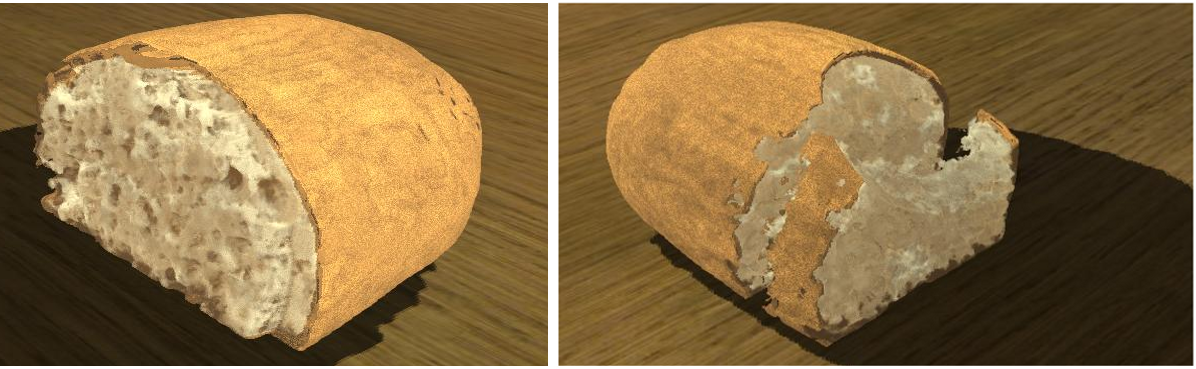
\includegraphics[width=13cm]{figures/otherbread}
\caption{Sliced breads after baking, using a scalar field of dimensions $256^{3}$. The images show that crumb and crust are taken into account in our approach.}
\label{fg:renders}
\end{center}
\end{figure*}

\begin{figure*}[!ht]
\begin{center}
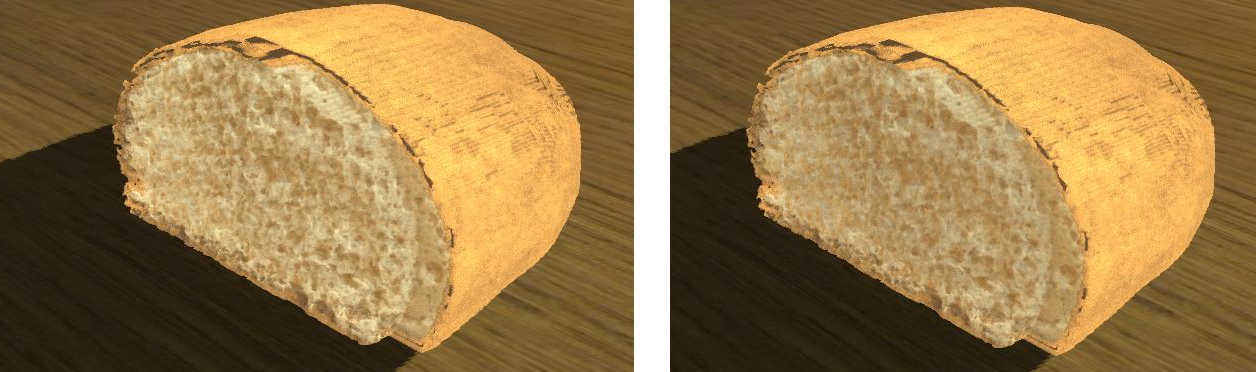
\includegraphics[width=13cm]{figures/otherbread512}
\caption{Sliced breads after baking, using a scalar field of dimensions $512^{3}$. Finer details can be seen in the crumb, augmenting the image quality.}
\label{fg:renders2}
\end{center}
\end{figure*}

\begin{figure*}[!ht]
\begin{center}
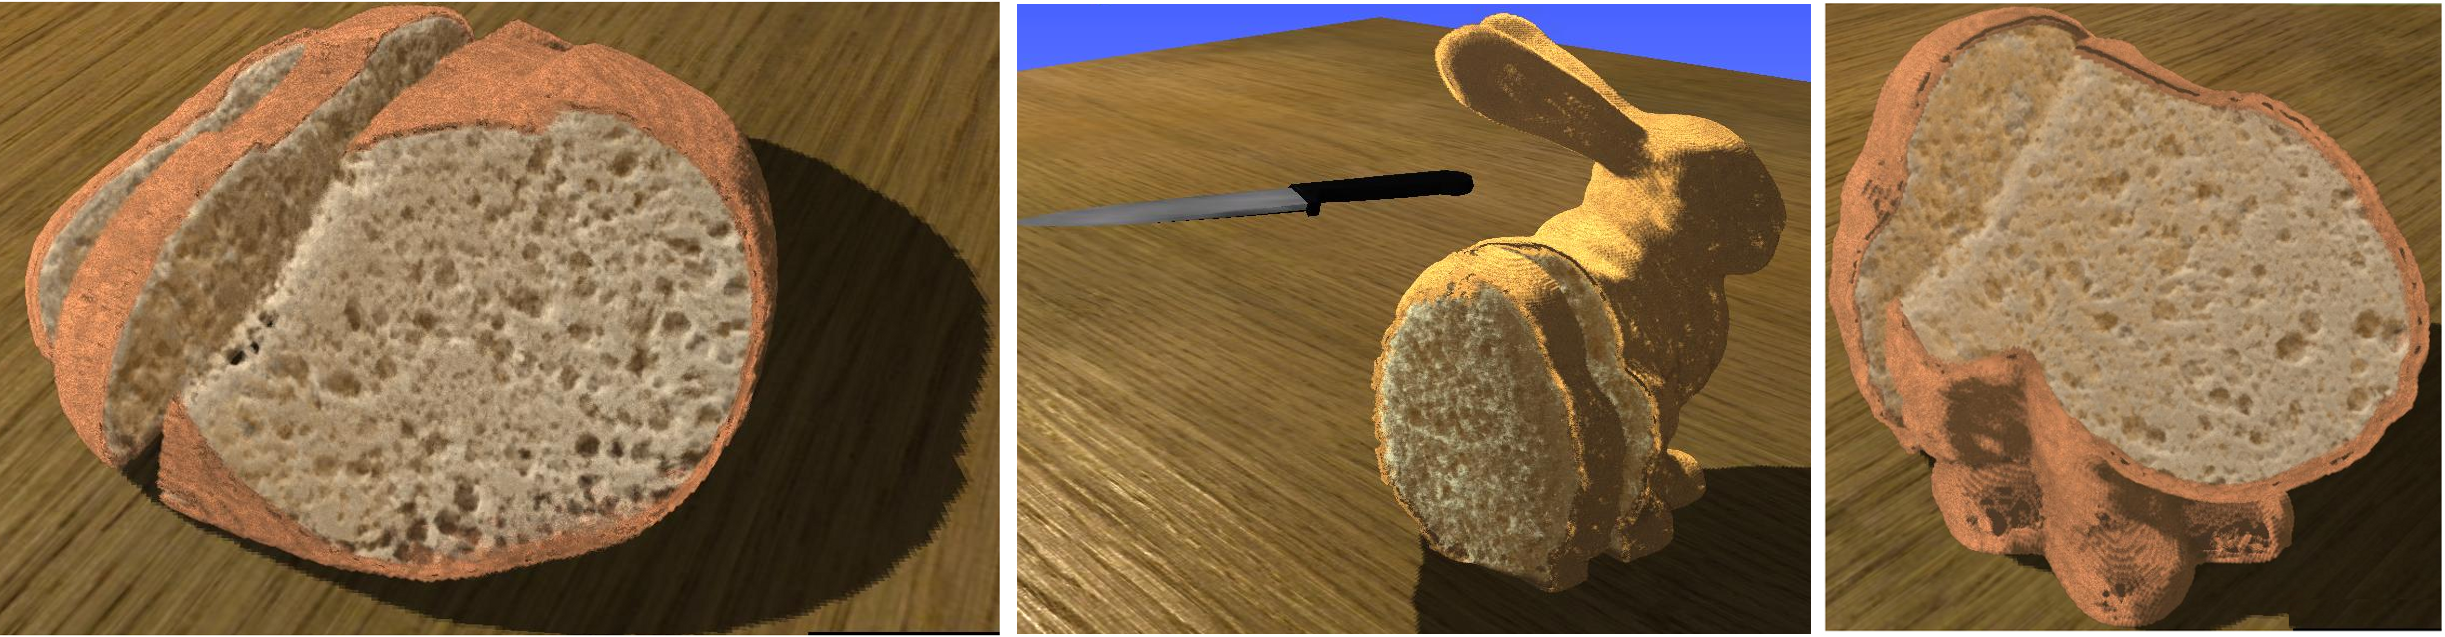
\includegraphics[width=13cm]{figures/final}
\caption{Sliced breads after baking. This image shows different $3D$ geometries.}
\label{fg:renders3}
\end{center}
\end{figure*}

\begin{figure*}[!ht]
\begin{center}
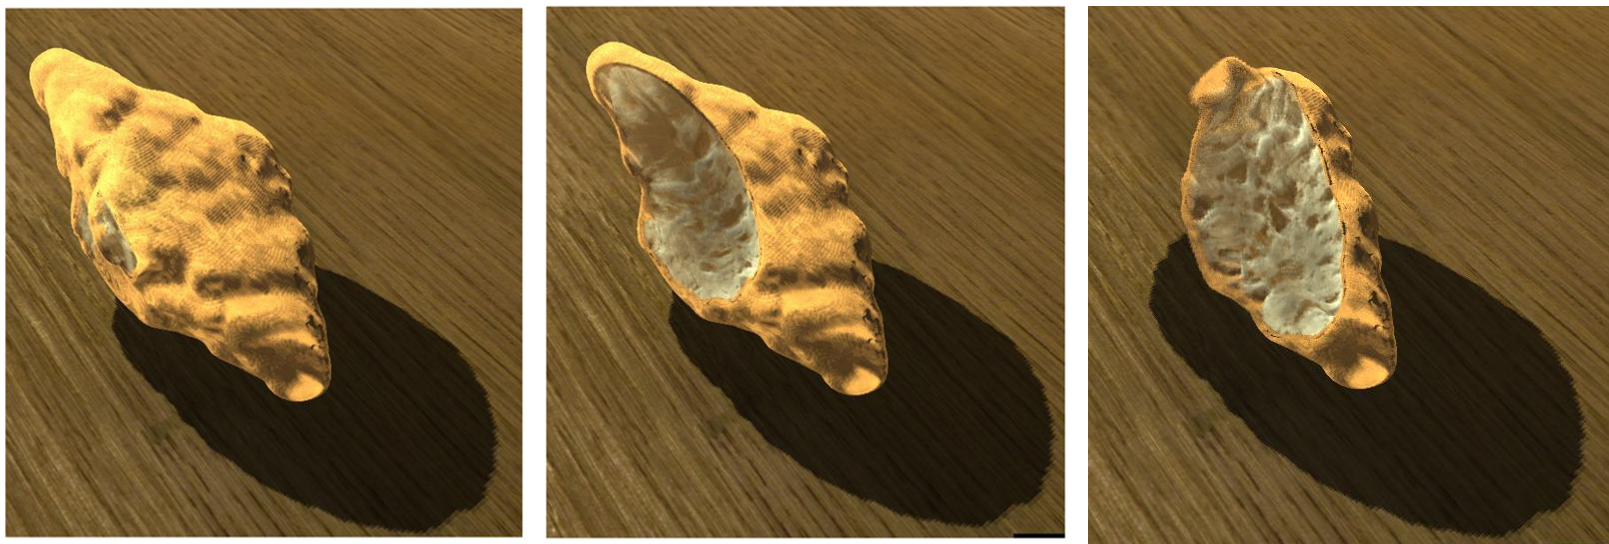
\includegraphics[width=13cm]{figures/croissant}
\caption{Sliced croissant after baking. This image shows the interior of the croissant at different volume regions.}
\label{fg:croissant}
\end{center}
\end{figure*}

\begin{figure*}[!ht]
\begin{center}
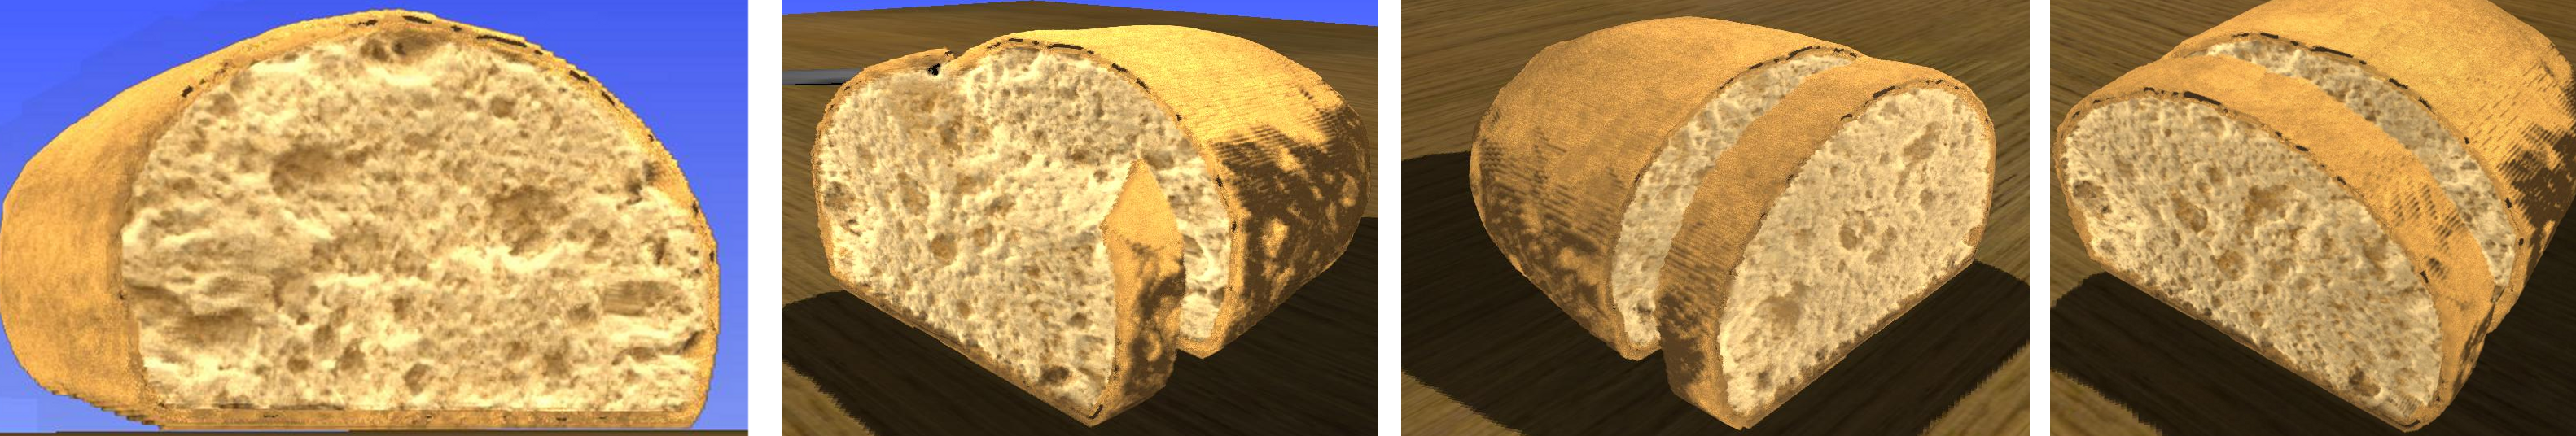
\includegraphics[width=13cm]{figures/baked}
\caption{Sliced breads after baking showing big alveoli typical of real breads.}
\label{fg:bigalveoli}
\end{center}
\end{figure*}

\begin{figure*}[!ht]
\begin{center}
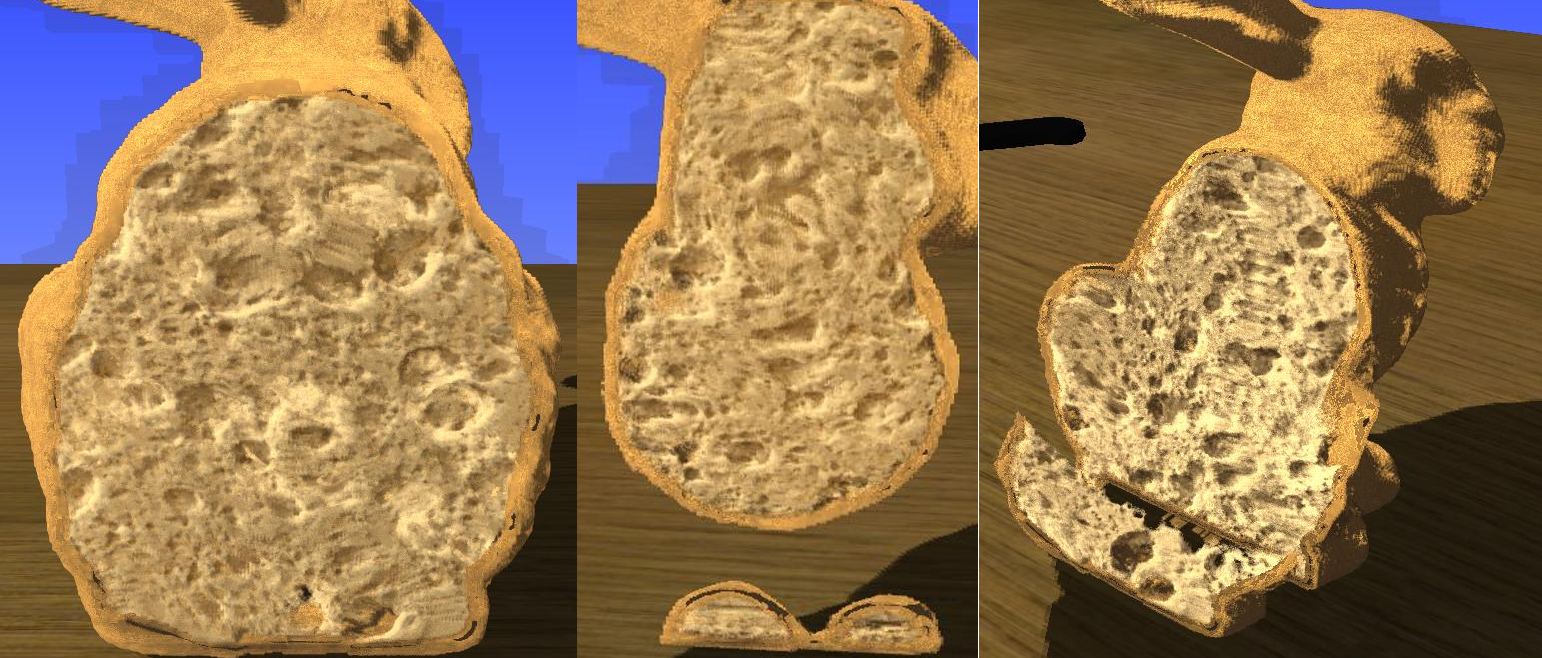
\includegraphics[width=13cm]{figures/bakedbunny}
\caption{Sliced breads after baking showing big alveoli typical of real breads. Also, the baking effect is clearly visible: bubbles tend to follow the crust shape.}
\label{fg:bakedbunny}
\end{center}
\end{figure*}


We used Python\footnote{python.org} and Cython\footnote{cython.org} for the implementation.
%Cython accelerates Python code using C-extensions
In Table~\ref{tab:computingtimes} we show typical times for the different processes in the bread making pipeline. In addition, rendering times with DVR are around $0.3$ seconds, achieving interactive framerates.

\begin{table}[h!]
       % Give a unique label
% For LaTeX tables use
\begin{tabular}{lllll}
\hline\noalign{\smallskip}
Scalar Field Resolution & $256^{3}$ & $384^{3}$  & $512^{3}$ \\
\noalign{\smallskip}\hline\noalign{\smallskip}
Proving & 0.28 & 0.97 & 2.29 \\
Intersection & 8 & 10.81 & 14.97 \\
Distance Field & 7 & 23.73 & 56 \\
Baking & 19.92 & 51.15 & 117.27 \\
%Rendering & 1s & 4s & 0\% \\
\noalign{\smallskip}\hline
\end{tabular}
\caption{Typical computing times in our pipeline expressed in seconds.}
\label{tab:computingtimes}
\end{table}


It is worth mention that most of the baking time is dedicated to the gradient computation and not the baking itself.
The user can generate previews using lower resolution scalar fields, avoiding high computing times when testing different bubble distributions and dough shapes.

%====================================================================
\section{Discussion}

To the best of the authors' knowledge, this is the first attempt in computer graphics to comprehensively model bread geometry using a physical model of bread baking.
Previous work in bread geometry computation involved advanced tomography equipment \cite{VanDyck2014} or artistic considerations \cite{Xenakis2007}.
These works are usually incomplete or inflexible to work with different bread types.
To overcome these difficulties, our pipeline comprises different stages simulating bread making that allow a flexible and versatile modeling. 
This allows to fine tune and test each step separately.
Several bread types can be simulated by simply setting appropriate parameters for external shapes and the dough texture.
This method allows to approximate the geometry of any real bread crumb, by 
extracting parameters in order to accurately simulate it.
The choice of geometry representation through scalar fields provided a flexible approach that allows to define the final shape, and to perform arbitrary cuts and slices in the geometries.

The proving step was inspired by visual similarities with Mandelbrot's model \cite{Mandelbrot1982}.
These patterns can be seen in several other porous materials such as foams, sponges, cheese, and many other.
Users can define different parameters related to the amount of bubbles, their radii, and their mutual relationship, obtaining a flexible framework for porous geometries.
The main visual difference between synthetic and real bread is that in the latter the bubbles in the crumb seldom intersect.
Even though it is feasible to modify our dough generating algorithm to include a bubble self-avoiding feature, the computational cost would be too high.

A $1D$ baking model was employed, but generalized to fit $3D$ geometries using a distance field, which retained the correctness and realism of the model.
This choice does not seem to impair the quality of the results, reducing the model complexity and the computing resources consumed. 
The warping induced by the baking step shows acceptable results in the global and local deformations exerted to the dough texture.
Also, since we physically emulated key steps in bread making, bubbles' shape adapted to the bread exterior silhouette, producing convincing patterns.

%Further analysis might be useful for richer characterizations.

%These experiments suggests that further research can be conducted for determining automatic parameters for a given real bread type.



%The use of a DVR engine produces realistic images and allowed to test the suitability of our model. Other photo-realistic algorithms can be used to test the capabilities of our method.

%====================================================================
%====================================================================
%====================================================================
\section{Conclusions}

In this chapter we introduced several algorithms to help close the gap of flexible and intuitive procedures in modeling some materials, particularly bread and other porous structures.
In addition, as a research subproduct, we obtained bidimensionals representations (textures) of wood, marble, and other materials than usually appears in the literature.
We visually demonstrated the feasibility of our methods.

As said, the first contribution of our work is an algorithm that outputs textures of several natural materials, using particle systems.
This work was presented at a local conference \cite{Baravalle2011}.

Our second contribution targets porous materials, particularly bread.
We designed algorithms based on particle systems in conjunction with dynamical systems to produce promising geometries of these materials.
This was presented at a local congress, and in a national publication \cite{Baravalle2014}.

Finally, and implementing an algorithm that is inspired in real bread formation, we employed knowledge from food engineering to design a pipeline that emulates the actual process of bread formation.
It allows to model arbitrary geometries of breads using a fractal generation algorithm.
The pipeline consists of a chained sequence of emulated real steps.
The proving step is defined by the user in two ways: the bread global shape is determined feeding a $3D$ model to the pipeline, and the bread local features are determined by setting different bubble distributions parameters (maximum and minimum bubble sizes, amount of bubbles, etc.).
A physical simulation of the baking process slightly warps the proved dough.
Finally, the crust is generated around the exterior of the baked volume.
The results were generated applying direct volume rendering, producing realistic images of crumb and crust for several bread types.
This pipeline is far more flexible and powerful than other state-of-the-art approaches for modeling bread geometry.

In a further chapter, we will show that the geometries produced by our pipeline are statistical coincident with real breads' geometries.


